\documentclass[a4paper]{article}
\usepackage{cmap}
\usepackage[utf8]{inputenc}
\usepackage[T2A]{fontenc}
\usepackage[english,russian]{babel} 
\usepackage[left=15mm, top=15mm, right=15mm, bottom=42mm, nohead, nofoot]{geometry}
\usepackage{blindtext}  % рыба-текст
\usepackage{graphicx}  % изобржаения
\usepackage{float} % плавающие объекты
\usepackage{wrapfig}  % изобржаения
\usepackage{tikz} % графика
\usepackage{mdframed} % рамки
\usepackage{xcolor} % определение цветов
\usepackage{nicefrac} % красивые дроби
\usepackage{cancel} % сокращение
\usepackage{amsmath,amsfonts,amssymb} % математический пакет
\usepackage{hyperref}  % гиперссылки
\usepackage{fancybox,fancyhdr} % хедер и футер
\usepackage{listings} % код
\pagestyle{fancy}
\fancyhf{}
\fancyhead[L]{Лабораторная работа №1}
\fancyhead[R]{\textit{Гистограммы, профили и проекции}}
\fancyfoot[C]{\thepage}
\headsep=8mm
\footskip=20mm

\definecolor{urlcolor}{HTML}{3454D1}
\definecolor{linkcolor}{HTML}{3454D1}
\hypersetup{pdfstartview=FitH, linkcolor=linkcolor, urlcolor=urlcolor, colorlinks=true}

\definecolor{strings}{rgb}{0,0.6,0}
\definecolor{comments}{rgb}{0,0.3,0}
\definecolor{numbers}{rgb}{0.5,0.5,0.5}
\definecolor{keywords}{rgb}{0.09,0.61,0.95}
\definecolor{background}{rgb}{0.97,0.97,0.97}
\lstdefinestyle{codestyle}{
    backgroundcolor=\color{background},
    commentstyle=\color{comments},
    keywordstyle=\color{keywords},
    stringstyle=\color{strings},
    numberstyle=\tiny\color{numbers},
    basicstyle=\ttfamily\footnotesize,
    breakatwhitespace=false,
    breaklines=true,
    captionpos=b,
    inputencoding=utf8,
    keepspaces=true,
    numbers=left,
    numbersep=5pt,
    showspaces=false,
    showstringspaces=false,
    showtabs=false,
    tabsize=2,
    extendedchars=true,
    literate=
    {а}{{\cyra}}1
    {б}{{\cyrb}}1
    {в}{{\cyrv}}1
    {г}{{\cyrg}}1
    {д}{{\cyrd}}1
    {е}{{\cyre}}1
    {ж}{{\cyrzh}}1
    {з}{{\cyrz}}1
    {и}{{\cyri}}1
    {й}{{\cyrishrt}}1
    {к}{{\cyrk}}1
    {л}{{\cyrl}}1
    {м}{{\cyrm}}1
    {н}{{\cyrn}}1
    {о}{{\cyro}}1
    {п}{{\cyrp}}1
    {р}{{\cyrr}}1
    {с}{{\cyrs}}1
    {т}{{\cyrt}}1
    {у}{{\cyru}}1
    {ф}{{\cyrf}}1
    {х}{{\cyrh}}1
    {ц}{{\cyrc}}1
    {ч}{{\cyrch}}1
    {ш}{{\cyrsh}}1
    {щ}{{\cyrshch}}1
    {ъ}{{\cyrhrdsn}}1
    {ы}{{\cyrery}}1
    {ь}{{\cyrsftsn}}1
    {э}{{\cyrerev}}1
    {ю}{{\cyryu}}1
    {я}{{\cyrya}}1
    {А}{{\CYRA}}1
    {Б}{{\CYRB}}1
    {В}{{\CYRV}}1
    {Г}{{\CYRG}}1
    {Д}{{\CYR96}}1
    {Е}{{\CYRE}}1
    {Ж}{{\CYRZH}}1
    {З}{{\CYRZ}}1
    {И}{{\CYRI}}1
    {Й}{{\CYRISHRT}}1
    {К}{{\CYRK}}1
    {Л}{{\CYRL}}1
    {М}{{\CYRM}}1
    {Н}{{\CYRN}}1
    {О}{{\CYRO}}1
    {П}{{\CYRP}}1
    {Р}{{\CYRR}}1
    {С}{{\CYRS}}1
    {Т}{{\CYRT}}1
    {У}{{\CYRU}}1
    {Ф}{{\CYRF}}1
    {Х}{{\CYRH}}1
    {Ц}{{\CYRC}}1
    {Ч}{{\CYRCH}}1
    {Ш}{{\CYRSH}}1
    {Щ}{{\CYRSHCH}}1
    {Ъ}{{\CYRHRDSN}}1
    {Ы}{{\CYRERY}}1
    {Ь}{{\CYRSFTSN}}1
    {Э}{{\CYREREV}}1
    {Ю}{{\CYRYU}}1
    {Я}{{\CYRYA}}1
}

\lstset{style=codestyle}

\addto\captionsrussian{
  \renewcommand{\contentsname}
    {\centering Содержание}
}
\newcommand{\addsection}[1]{
    \phantomsection
    \addcontentsline{toc}{section}{#1}
    \section*{\centering #1}
}
\newcommand{\addsubsection}[1]{
    \phantomsection
    \addcontentsline{toc}{subsection}{#1}
    \subsection*{\centering #1}
}
\newcommand{\addsubsubsection}[1]{
    \phantomsection
    \addcontentsline{toc}{subsubsection}{#1}
    \subsubsection*{\centering #1}
}

\newmdenv[
  leftmargin = 0.5em,
  skipabove = 0.5em,
  skipbelow = 0.5em,
  linewidth = 1pt,
  rightline = false,
  topline = false,
  bottomline = false
]{quotebox}

\newlength{\tempheight}
\newcommand{\Let}{
\mathbin{\text{\settoheight{\tempheight}{\mathstrut}\raisebox{0.4\pgflinewidth}{
\tikz[baseline=0.5ex,line cap=round,line join=round] \draw (0,0) --++ (0.3em,0) --++ (0,2.3ex) --++ (-0.3em,0);
}}}}
\newcommand*\squared[1]{\tikz[baseline=(char.base)]{
            \node[shape=rectangle,draw,inner sep=4pt] (char) {#1};}}
\newcommand*\msquared[1]{\tikz[baseline=(char.base)]{
            \node[shape=rectangle,draw,inner sep=4pt] (char) {$\displaystyle #1$};}}
\newcommand{\at}{\biggr\rvert}
\newcommand{\shiftright}[3]{\makebox[#2][r]{\makebox[#1][l]{#3}}}
\newcommand{\e}{\;\text{e}}
\let\oldint\int
\def\int{\oldint\limits}
\DeclareRobustCommand{\divby}{%
  \mathrel{\vbox{\baselineskip.65ex\lineskiplimit0pt\hbox{.}\hbox{.}\hbox{.}}}%
}

\newcommand\NB{\textbf{N\kern-0.32em\textcolor{red}{B}}}

\begin{document}

\begin{titlepage}
    \begin{center}
        Федеральное государственное автономное образовательное \\ учреждение высшего образования \\[6pt]
        САНКТ-ПЕТЕРБУРГСКИЙ НАЦИОНАЛЬНЫЙ \\ ИССЛЕДОВАТЕЛЬСКИЙ УНИВЕРСИТЕТ ИТМО \\[16pt]
        Факультет систем управления и робототехники \\[26em]
        Лабораторная работа №1 \\[0.5em]
        \textbf{ГИСТОГРАММЫ, ПРОФИЛИ И ПРОЕКЦИИ}
    \end{center}\,\\[10em]
    \begin{flushright}
        Студенты: Овчинников П.А.\\
        Румянцев А.А.\\
        Чебаненко Д.А.\\[0.7em]
        Поток: ТЕХ.ЗРЕНИЕ 2.1 \\[0.7em]
        Преподаватель: Шаветов С.В.
    \end{flushright}\,\\[4.8em]
    \begin{center}
        {\small Санкт-Петербург \\ 2024}
    \end{center}
\end{titlepage}
\setcounter{page}{2}
\tableofcontents\newpage
\addsection{Цель работы}
В этой работе мы изучим основные яркостные и геометрические характеристики изображений, чтобы использовать их для анализа изображения. Мы научимся вычислять гистограммы, профили и проекции изображений, чтобы в дальнейшем использовать их в других задачах вне лабораторной работы.
\addsection{Код, используемый в работе}
Для начала стоит отметить, что весь код опубликован в \href{https://gist.github.com/PaveTranquil/64ed1c48f4faa3a25f826c5f00c7ab5f}{приватном гисте в GitHub}, доступном только по ссылке из этого отчёта. Часть кода будет приведена под этим заголовоком с указанием необходимых импортов, и остальная часть будет приведена в соответствующих разделах отчёта уже без указания импортов для экономия места.

\addsubsection{Вычисление гистограмм}
\begin{lstlisting}[language=Python, caption=Вычисление нормализованных RGB- и кумулятивных гистограмм]
from typing import Sequence
import cv2
from cv2.typing import MatLike
import numpy as np
from numpy._typing import NDArray


def calc_rgb_hist(channels: Sequence[MatLike]) -> list[MatLike]:
    """Вычисляет нормализованные гистограммы изображения"""
    hists = []
    for i in range(3):
        hist = cv2.calcHist(channels, [i], None, [hist_size], hist_range)
        hists.append(hist / (image.shape[0] * image.shape[1]))  # Нормализуем гистограмму
    return hists


def calc_cumulative_hist(channels: Sequence[MatLike]) -> tuple[NDArray, ...]:
    """Вычисляет кумулятивную гистограмму изображения"""
    # Подсчитываем гистограммы по каналам, применяем к ним np.cumsum и возвращаем в кортеже
    return tuple(map(np.cumsum, calc_rgb_hist(channels)))
\end{lstlisting}
Перед вами две функции, одна из которых подсчитывает нормализованную RGB-гистограмму, а вторая использует первую, чтобы подсчитать кумулятивную гистограмму по каждому из каналов. В обоих случаях используется библиотека \verb|OpenCV| для работы с изображениями и библиотека \verb|NumPy| для работы с массивами. Функция, вычисляющая кумулятивную гистограмму, будет активно использоваться в течение всей лабораторной работы.

\addsubsection{Отрисовка гистограмм и изображения}
\begin{lstlisting}[language=Python, caption=Отрисовка RGB- и кумулятивной гистограмм]
from typing import Callable, Sequence
import cv2
from cv2.typing import MatLike
import matplotlib.pyplot as plt
import numpy as np


def clear():
    """Очищает холст matplotlib от графиков"""
    plt.cla()  # Очищаем график
    plt.clf()  # Очищаем фигуру
    plt.subplots_adjust(left=0.07, right=0.95)


def render_rgb_hist(channels: Sequence[MatLike], name: str):
    """Рендерит гистограмму изображения из нормализованных гистограмм каждого канала"""
    clear()
    hists = calc_rgb_hist(channels)

    plt.grid(True)
    plt.xlim(hist_range)
    plt.ylim(-0.001, 0.1)
    for hist, color in zip(hists[::-1], ('r', 'g', 'b')):
        plt.plot(hist, color=color)

    plt.title('RGB-гистограма')
    plt.savefig(f'{name}.png')


def render_cumulative_hist(channels: Sequence[MatLike], name: str):
    """Рендерит кумулятивную гистограмму изображения"""
    clear()
    cumhists = calc_cumulative_hist(channels)

    plt.grid(True)
    plt.xlim(hist_range)
    plt.ylim(-0.005, 1.005)
    for hist, color in zip(cumhists[::-1], ('r', 'g', 'b')):
        plt.plot(hist, color=color)

    plt.title('Кумулятивная гистограмма')
    plt.savefig(f'{name}.png')


def apply_method(method: Callable, image: MatLike, output_dir: str, **kwargs):
    """Применяет преобразование к изображению, компрессирует значения выше
    максимальной яркости до 255 и сохраняет результат в папку output_dir"""
    new_image = method(image, **kwargs)
    cv2.threshold(new_image, 255, 255, cv2.THRESH_TRUNC, new_image)
    new_image = new_image.astype(np.uint8)
    cv2.imwrite(f'{output_dir}/photo.jpg', new_image)

    # Отрендерим гистограммы преобразованного изображения
    render_rgb_hist(cv2.split(new_image), f'{output_dir}/hist')
    render_cumulative_hist(cv2.split(new_image), f'{output_dir}/cumhist')
\end{lstlisting}
Этот код отвечает за отрисовку гистограмм и изображений. В нём используется библиотека \verb|matplotlib| для отрисовки графиков. В функции \verb|clear| происходит очистка холста от предыдущих графиков, чтобы не возникало накладывания одних графиков на другие. Функции \verb|render_rgb_hist| и \verb|render_cumulative_hist| отвечают за отрисовку RGB- и кумулятивной гистограмм соответственно. В обоих случаях используются функции для посчёта гистограмм, которые были определены в предыдущем листинге.\\[0.5em]
Отдельного внимания заслуживает функция \verb|apply_method|, которая принимает на вход функцию \verb|method|, изображение \verb|image|, папку для сохранения результата и дополнительные аргументы, которые передаются вместе с изображением в \verb|method|. Затем функция применяет преобразование к изображению, компрессирует значения выше максимальной яркости до 255 (это нужно для того, чтобы избежать искажений, связанных с цикличным повторением гистограммы) и сохраняет результат в папку \verb|output_dir|. После этого она вызывает функции для отрисовки гистограмм уже преобразованного изображения, чтобы можно было сравнить гистограммы.\newpage


\addsection{Преобразование гистограммы изображения}
Перед началом работы с преобразованиями стоит продемонстрировать исходное изображение и его гистограммы.
\begin{figure}[H]
    \centering
    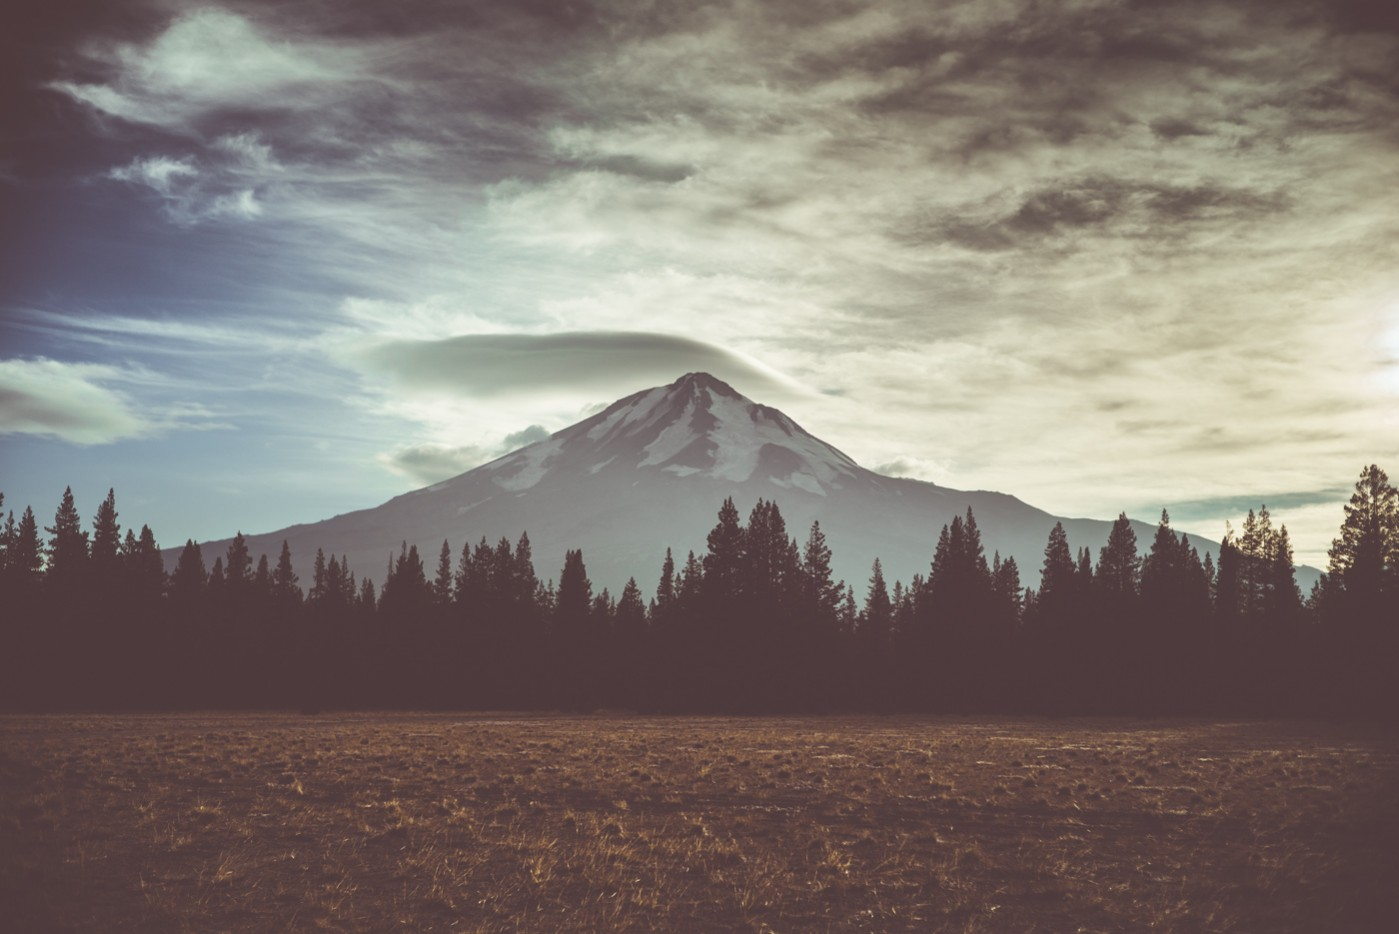
\includegraphics[width=0.7\textwidth]{images/photo.jpg}
    \caption{Исходное изображение}
    \begin{minipage}{0.5\textwidth}
        \centering 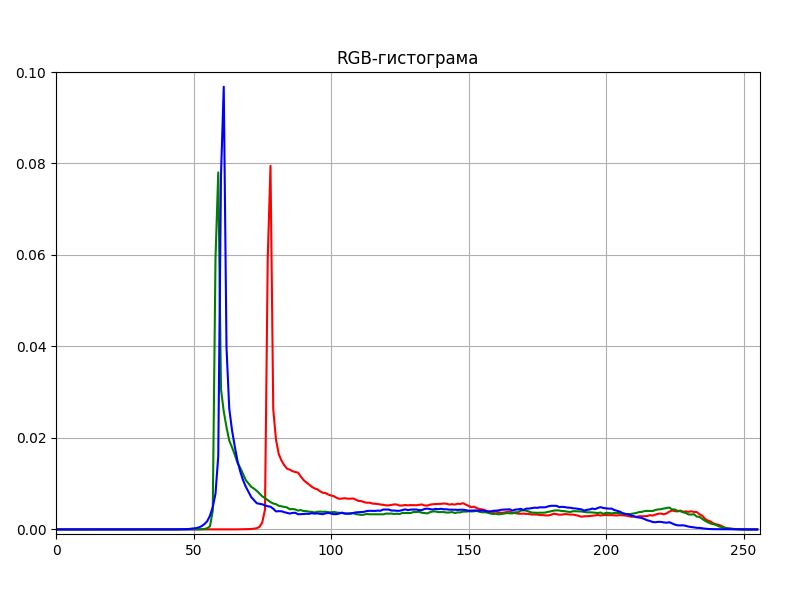
\includegraphics[width=\textwidth]{images/hist.png}
    \end{minipage}\hfill
    \begin{minipage}{0.5\textwidth}
        \centering 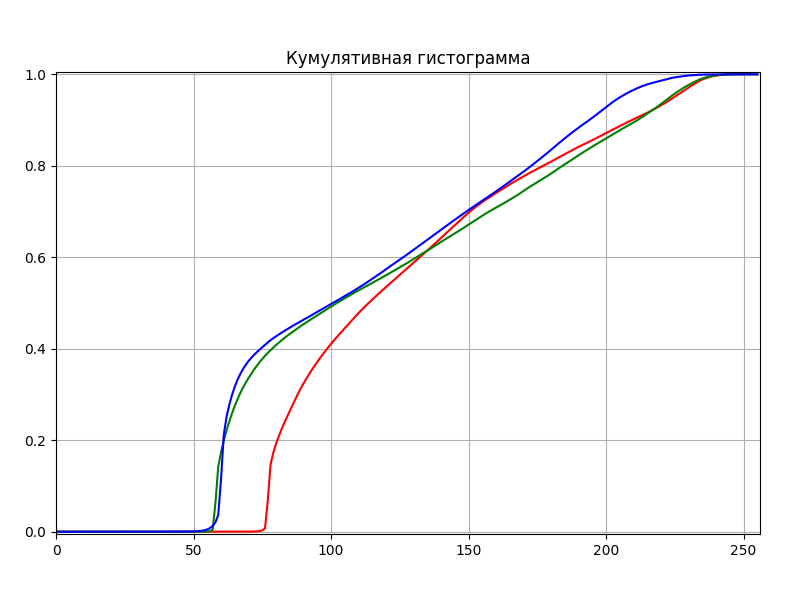
\includegraphics[width=\textwidth]{images/cumhist.png}
    \end{minipage}
\end{figure}\noindent
Итак, вот гистограммы исходного изображения, из которых можно сделать такие выводы:
\begin{itemize}
    \item На RGB-гистограмме видны три пика для каждого канала в тёмной части спектра
    \item Градации до 50-ти вовсе отсутствуют на изображении
    \item Изображение в общем и целом не очень яркое, что хорошо видно по обеим гистограммам на градациях выше 100.
\end{itemize}
Очевидно, это изображение хочет, чтобы мы навели в нём красоту, а значит мы готовы преобразовываться! Для каждого из преобразований будет приведён код функции, которая реализует его, а также код для запуска преобразования с помощью функции \verb|apply_method| для понимания того, какие коэффициенты передаются в функцию преобразования.


\newpage\addsubsection{Линейное выравнивание гистограммы}
\textbf{Линейное выравнивание} гистограммы требует наличия кумулятивной гистограммы, которая в свою очередь будет выравнена этим методом в прямую линию. Ниже код для этого преобразования:
\begin{lstlisting}[language=Python, caption={Код, реализующий линейное выравнивание гистограммы}]
def linear_alignment(image: MatLike) -> NDArray[np.uint8]:
    """Линейное выравнивание гистограммы"""
    channels = cv2.split(image)
    cumhists = calc_cumulative_hist(channels)
    new_channels = []  # Будем формировать новые каналы в этот список
    for channel, cumhist in zip(channels, cumhists):
        # Применяем линейное выравнивание к каждому каналу по кумулятивной гистограмме
        # В гистограмме диапазон [0..1], поэтому умножаем на 255
        new_channels.append(255 * cumhist[channel])
    return cv2.merge(new_channels)


apply_method(linear_alignment, image, '1aligned')
\end{lstlisting}
\begin{figure}[H]
    \centering
    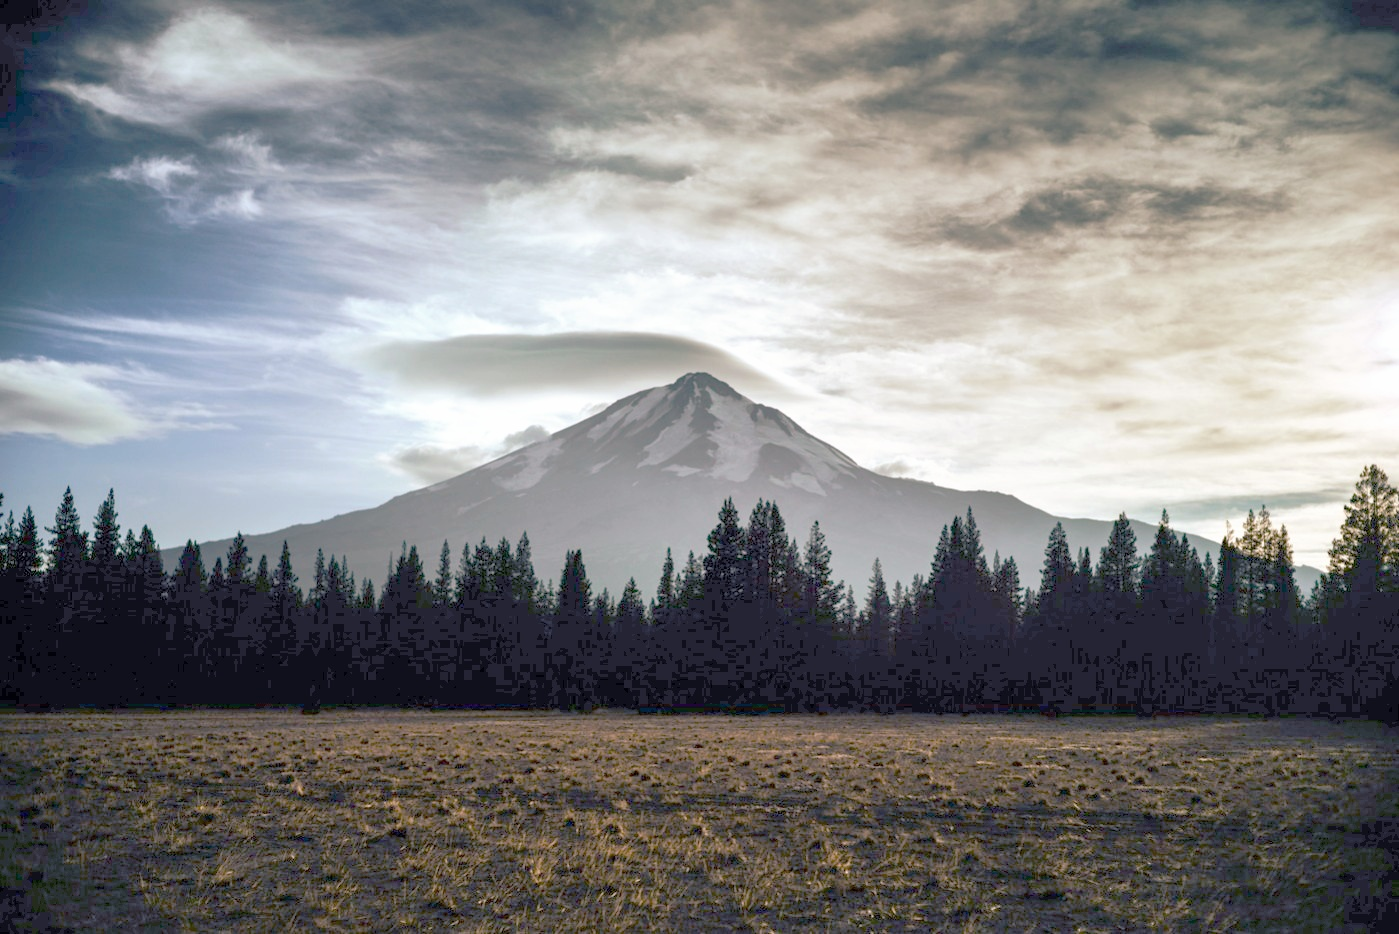
\includegraphics[width=0.57\textwidth]{images/1aligned/photo.jpg}
    \begin{minipage}{0.5\textwidth}
        \centering 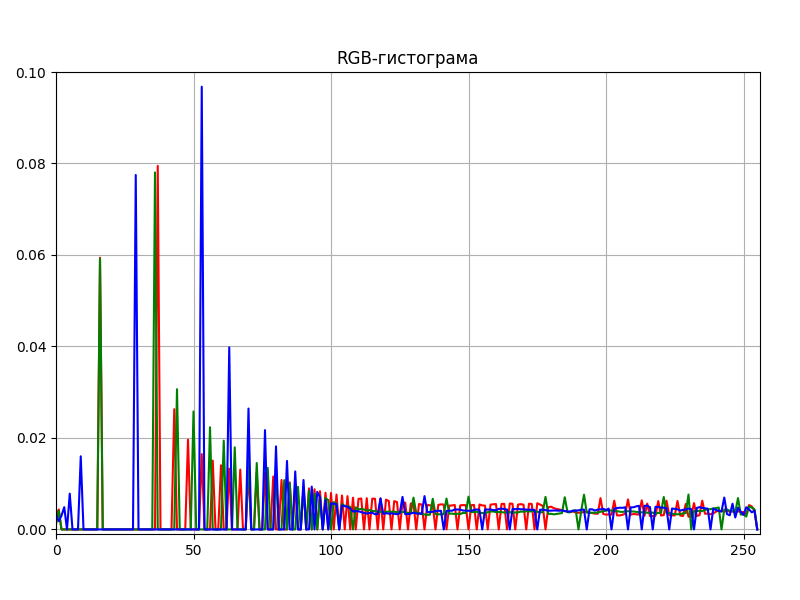
\includegraphics[width=\textwidth]{images/1aligned/hist.png}
    \end{minipage}\hfill
    \begin{minipage}{0.5\textwidth}
        \centering 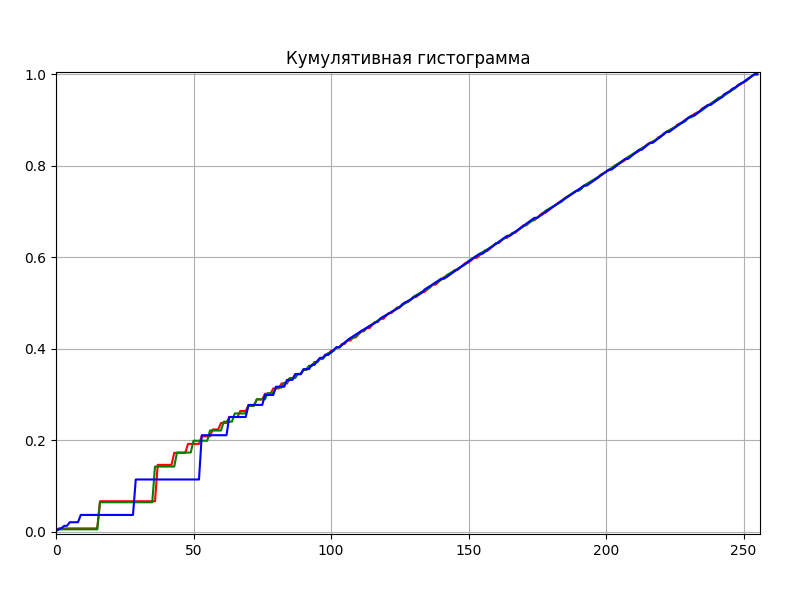
\includegraphics[width=\textwidth]{images/1aligned/cumhist.png}
    \end{minipage}
\end{figure}\noindent
И мы видим, что RGB-гистограмма изображения изменилась так, что теперь кумулятивная гистограмма выглядит как равномерная линия (в начале гистограммы наблюдаются скачки, связанные с низким качеством изображения). В целом, это преобразование натурализировало цвета изображения, избавив его от красноватого оттенка, и сделало его ярче. К тому же почти не заметна тёмная виньетка по краям изображения. И, самое главное, преобразование сделало это без засветов на небе --- мы всё ещё видим детали в облаках, это говорит о повышении контрастности.


\newpage\addsubsection{Арифметические операции}
Одно из простейших преобразований --- \textbf{арифметические операции}, т.е. добавление и вычитание какого-то количества градаций к каждому из каналов. Исходя из RGB-гистограммы первоначального изображения, устанавливаем сдвиг синего и зелёного канала на 65 градаций вправо, а сдвиг красного канала --- на 50 градаций вправо. Вот код для этого преобразования:
\begin{lstlisting}[language=Python, caption={Код, реализующий арифметические операции над изображением}]
def arithmetic_operations(image: MatLike, shifts: list[float]) -> NDArray[np.uint8]:
    """Арифметические операции с изображением"""
    channels = list(cv2.split(image))
    for i, channel in enumerate(channels):
        # Сдвигаем каждый канал на значение shift
        channels[i] = np.clip(channel.astype(np.uint16) + shifts[i], 0, 255).astype(np.uint8)
    return cv2.merge(channels)


apply_method(arithmetic_operations, image, '2shift', shifts=[65, 65, 50])
\end{lstlisting}
\begin{figure}[H]
    \centering
    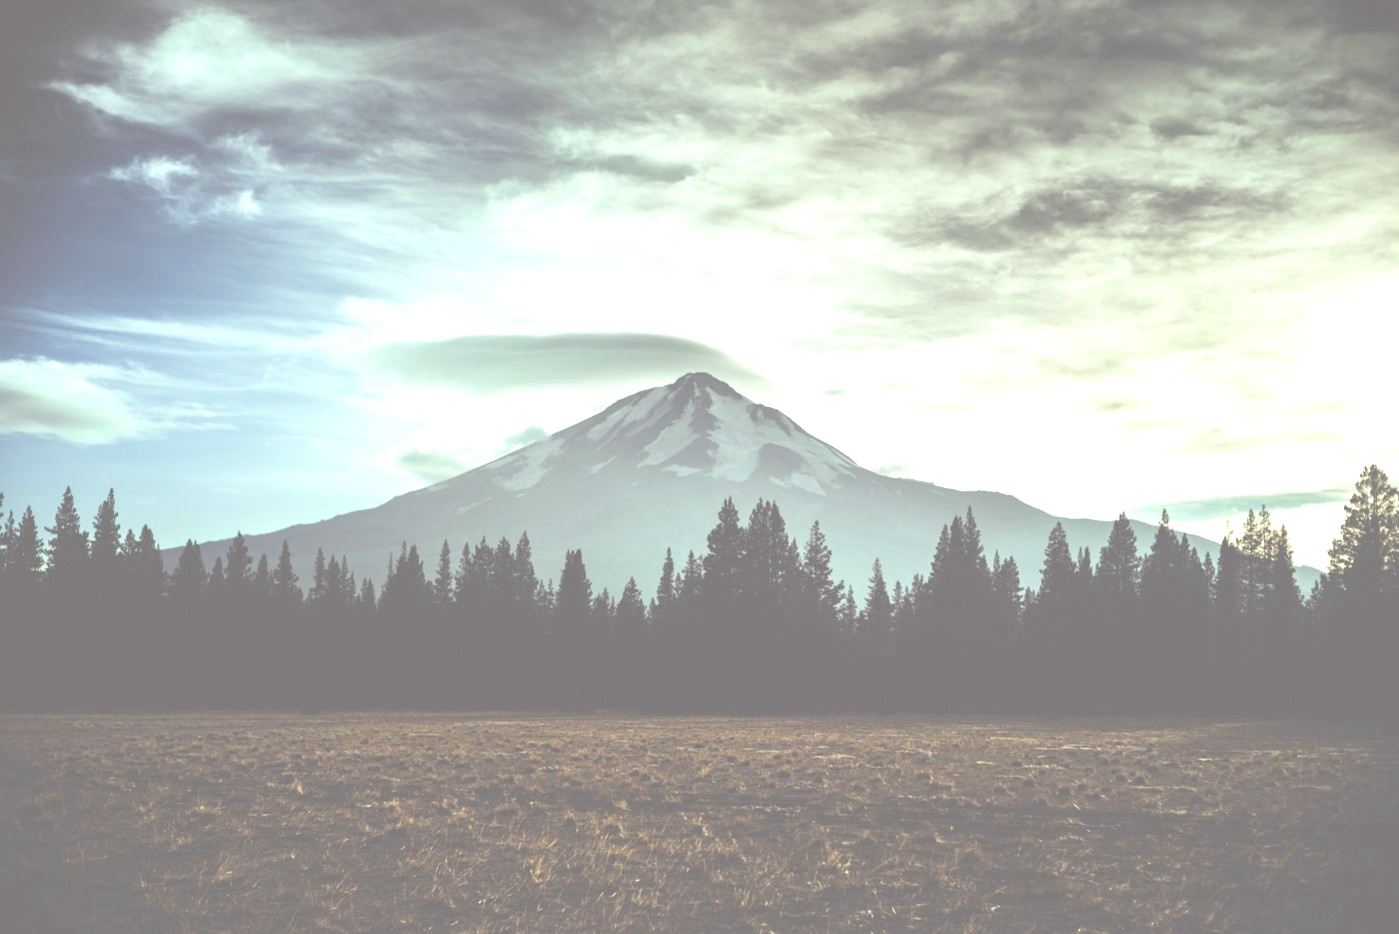
\includegraphics[width=0.56\textwidth]{images/2shift/photo.jpg}
    \begin{minipage}{0.5\textwidth}
        \centering 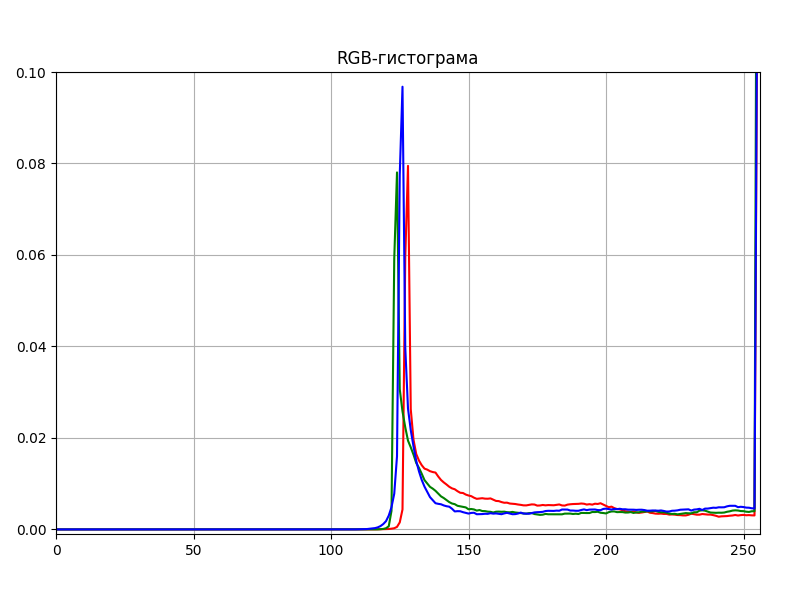
\includegraphics[width=\textwidth]{images/2shift/hist.png}
    \end{minipage}\hfill
    \begin{minipage}{0.5\textwidth}
        \centering 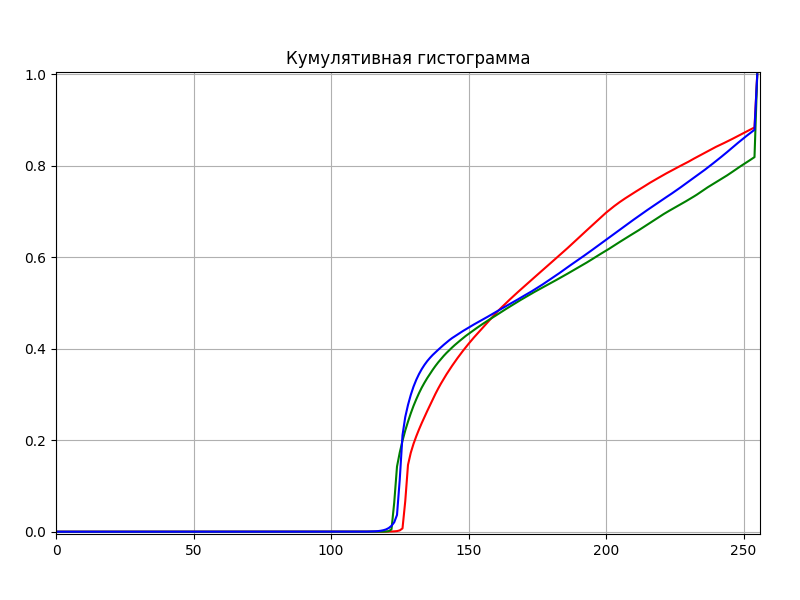
\includegraphics[width=\textwidth]{images/2shift/cumhist.png}
    \end{minipage}
\end{figure}\noindent
\NB: в коде происходит расширение типа данных до \verb|uint16| перед выполнением сдвига, чтобы избежать переполнения с цикличным сдвигом RGB-гистограммы --- так мы не будем наблюдать искажения в изображении.\\[0.5em]
Как мы видим, оттенок в изображении изменился и оно стало ярче, однако применение арифметических операций хоть и простое, но не прибавляет к изображению контрастности и не улучшаег визуально --- мы потеряли часть изображения в светлых участках, и теперь небо выглядит как однородная масса. Так что это преобразование не слишком практичное.


\newpage\addsubsection{Растяжение динамического диапазона}
\textbf{Растяжение динамического диапазона} --- отличное преобразование, которое расширяет сжатый диапазон до нуля и максимума с обоих сторон гистограммы. Нелинейность преобразования (которую мы заметим на кумулятивной гистограмме) регулируется с помощью коэффициента нелинейности $\alpha = 0.8$. И код перед вами:
\begin{lstlisting}[language=Python, caption={Код, растягивающий динамический диапазон изображения}]
def contrast_stretching(image: MatLike, alpha: float) -> NDArray[np.uint8]:
    """Расширение контраста методом растяжения динамического диапазона"""
    # Если изображение в целочисленном диапазоне [0..255], то конвертируем в вещественный [0..1]
    image = image.astype(np.float64) / 255 if image.dtype == 'uint8' else image
    channels = list(cv2.split(image))
    for i, channel in enumerate(channels):
        cmin, cmax = channel.min(), channel.max()
        channels[i] = ((channel - cmin) / (cmax - cmin)) ** alpha * 255
    image = cv2.merge(channels)
    # Если изображение было в целочисленном диапазоне, то возвращаем его обратно в этот диапазон
    return (image.clip(0, 255) if image.dtype == 'uint8' else image).astype(np.uint8)


apply_method(contrast_stretching, image, '3stretched', alpha=0.8)
\end{lstlisting}
\begin{figure}[H]
    \centering
    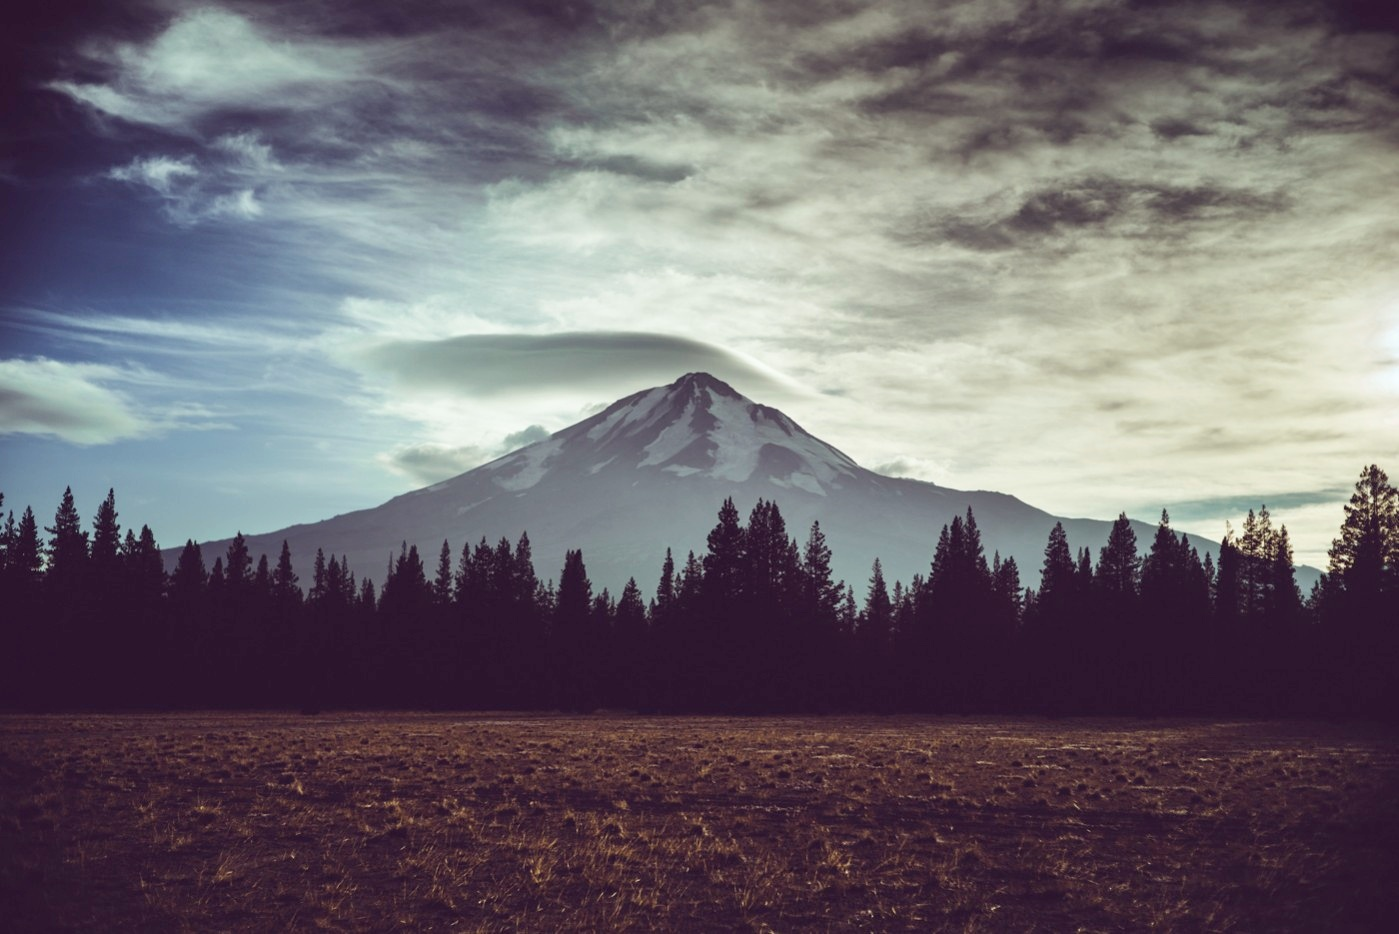
\includegraphics[width=0.56\textwidth]{images/3stretched/photo.jpg}
    \begin{minipage}{0.5\textwidth}
        \centering 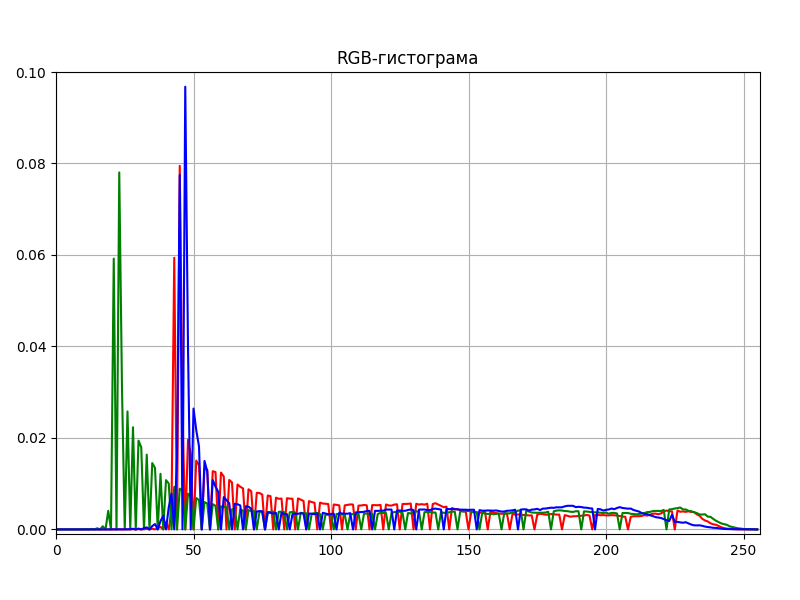
\includegraphics[width=\textwidth]{images/3stretched/hist.png}
    \end{minipage}\hfill
    \begin{minipage}{0.5\textwidth}
        \centering 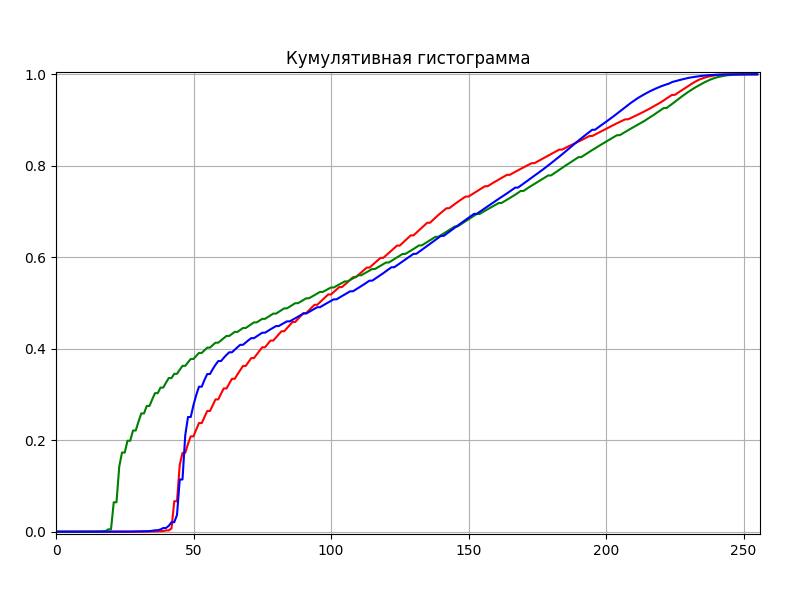
\includegraphics[width=\textwidth]{images/3stretched/cumhist.png}
    \end{minipage}
\end{figure}\noindent
Как мы видим, с изображения спала белая пелена выгорания, которая добавляла лишнюю яркость всему изображению --- из-за этого на небе видно больше деталей и в целом изображение стало более контрастным и сочным в цветах. Однако из-за нелинейности преобразования мы потеряли детали в тёмных участках изображения, и теперь ели выглядят как однородная масса. Преобразование подойдёт, чтобы сделать старые снимки с выгораниями лучше и убавить блики, но оно не очень хорошо работает на тёмных изображениях.


\newpage\addsubsection{Равномерное преобразование}
\textbf{Равномерное преобразование} отличается от линейного выравнивания тем, что оно не растягивает гистограмму в прямую линию, а делает её равномерной с самого тёмного пикселя каждого канала. Вот код для этого преобразования:
\begin{lstlisting}[language=Python, caption={Код, реализующий равномерное преобразование}]
def uniform_conversion(image: MatLike) -> NDArray[np.uint8]:
    """Равномерное преобразование гистограммы"""
    channels = cv2.split(image)
    cumhists = calc_cumulative_hist(channels)
    new_channels = []
    for channel, cumhist in zip(channels, cumhists):
        cmin, cmax = channel.min(), channel.max()
        new_channels.append((cmax - cmin) * cumhist[channel] + cmin)
    return cv2.merge(new_channels)


apply_method(uniform_conversion, image, '4uniform')
\end{lstlisting}
\begin{figure}[H]
    \centering
    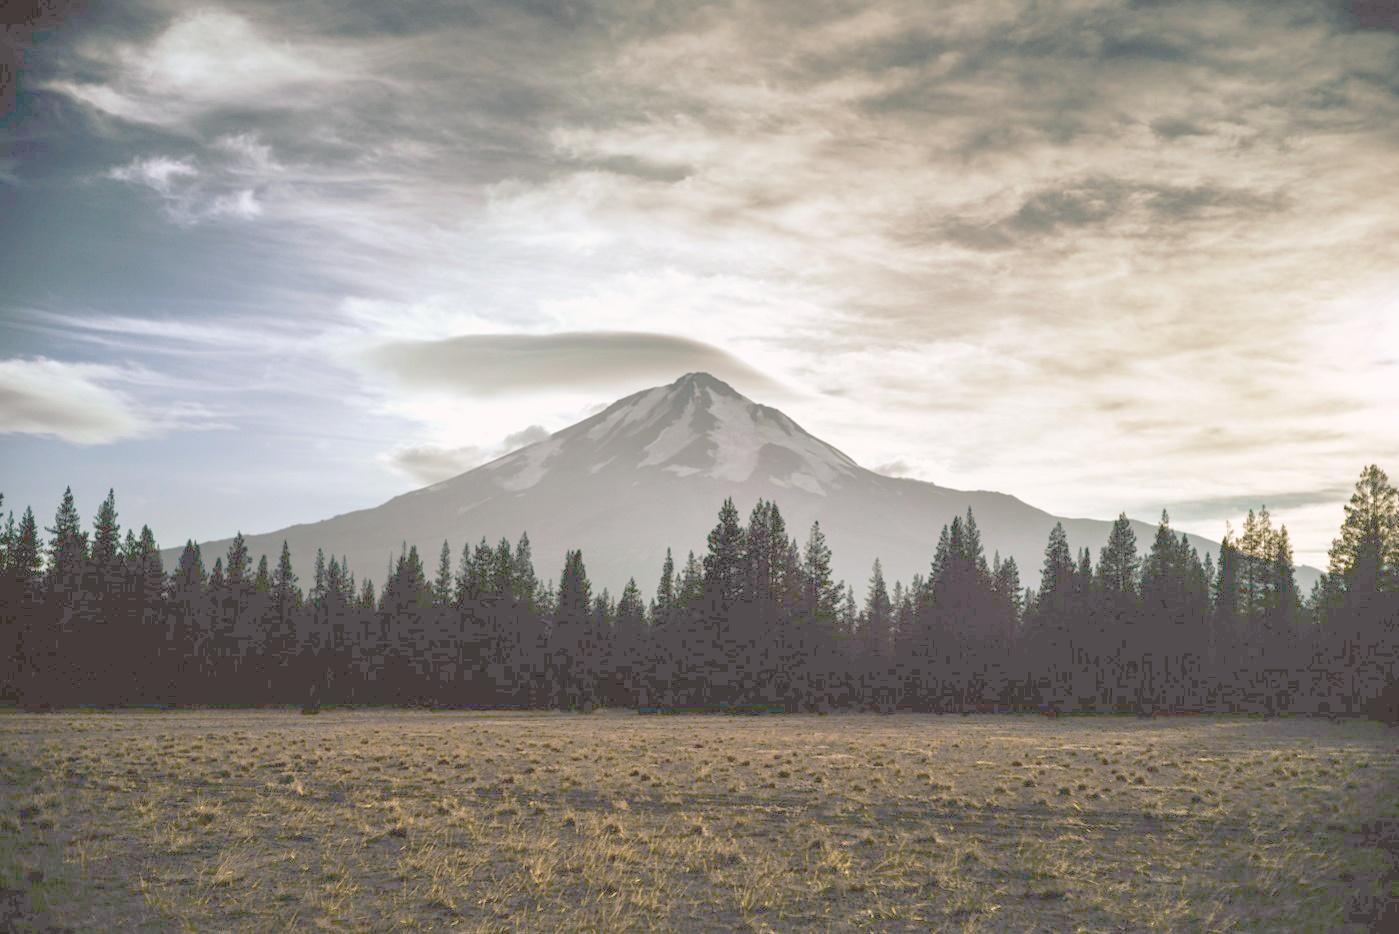
\includegraphics[width=0.56\textwidth]{images/4uniform/photo.jpg}
    \begin{minipage}{0.5\textwidth}
        \centering 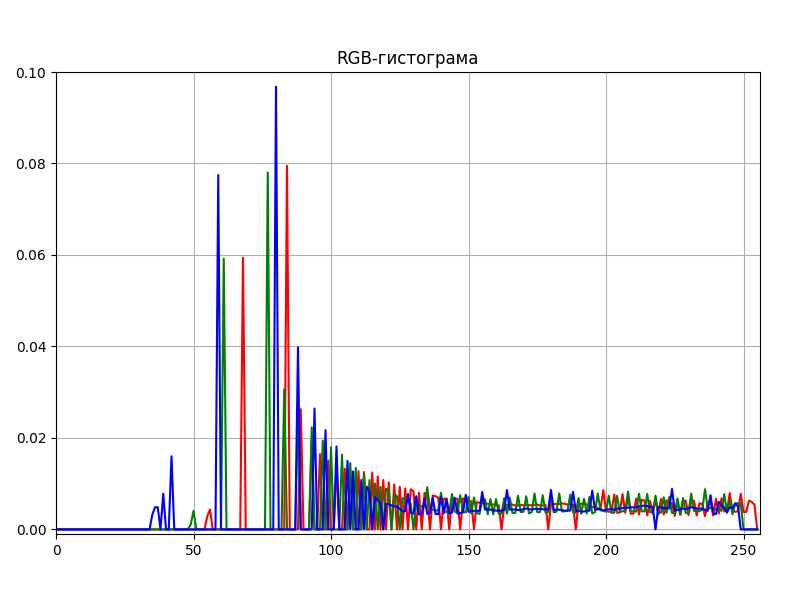
\includegraphics[width=\textwidth]{images/4uniform/hist.png}
    \end{minipage}\hfill
    \begin{minipage}{0.5\textwidth}
        \centering 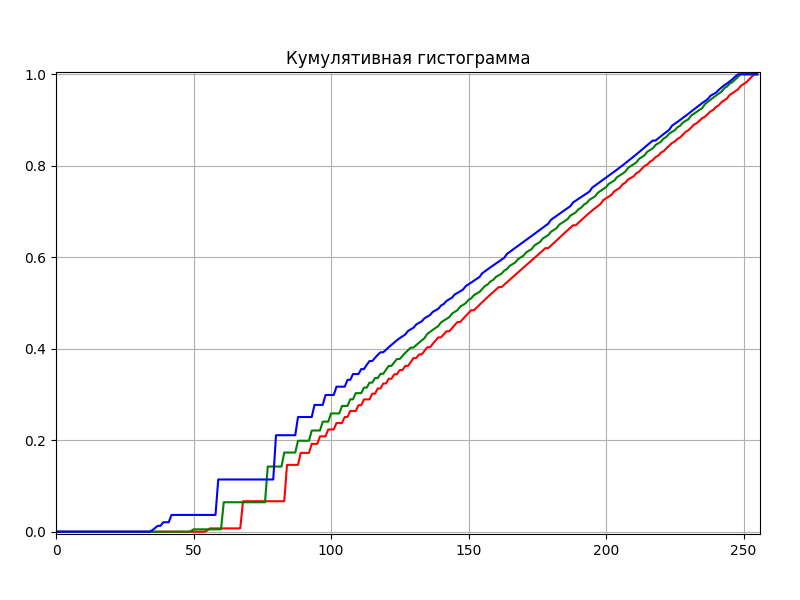
\includegraphics[width=\textwidth]{images/4uniform/cumhist.png}
    \end{minipage}
\end{figure}\noindent
Изображение стало более контрастным, и теперь на нём видно больше деталей в тёмных участках, но при этом яркость изображения не изменилась и по-прежнему наблюдается выгорание, однако тёмная виньетка вокруг изображения практически полностью устранена. Преобразование идеально подойдёт для тёмных изображений, но не для ярких, т.к. яркость изображения не меняется.


\newpage\addsubsection{Экспоненциальное преобразование}
\textbf{Экспоненциальное преобразование} --- это преобразование, которое подгоняет RGB-гистограмму так, что кумулятивная гистограмма становится экспоненциальной функцией, крутизну которой можно регулировать с помощью коэффициента $\alpha = 4$. Давайте взглянем на код:
\begin{lstlisting}[language=Python, caption={Код, реализующий экспоненциальное преобразование}]
def exponential_conversion(image: MatLike, alpha: float) -> NDArray[np.uint8]:
    """Экспоненциальное преобразование гистограммы"""
    channels = cv2.split(image)
    cumhists = calc_cumulative_hist(channels)
    new_channels = []
    for channel, cumhist in zip(channels, cumhists):
        cmin = channel.min()
        new_channels.append(cmin - 255 / alpha * np.log(1 - cumhist[channel]))
    return cv2.merge(new_channels)


apply_method(exponential_conversion, image, '5exponential', alpha=4)
\end{lstlisting}
\begin{figure}[H]
    \centering
    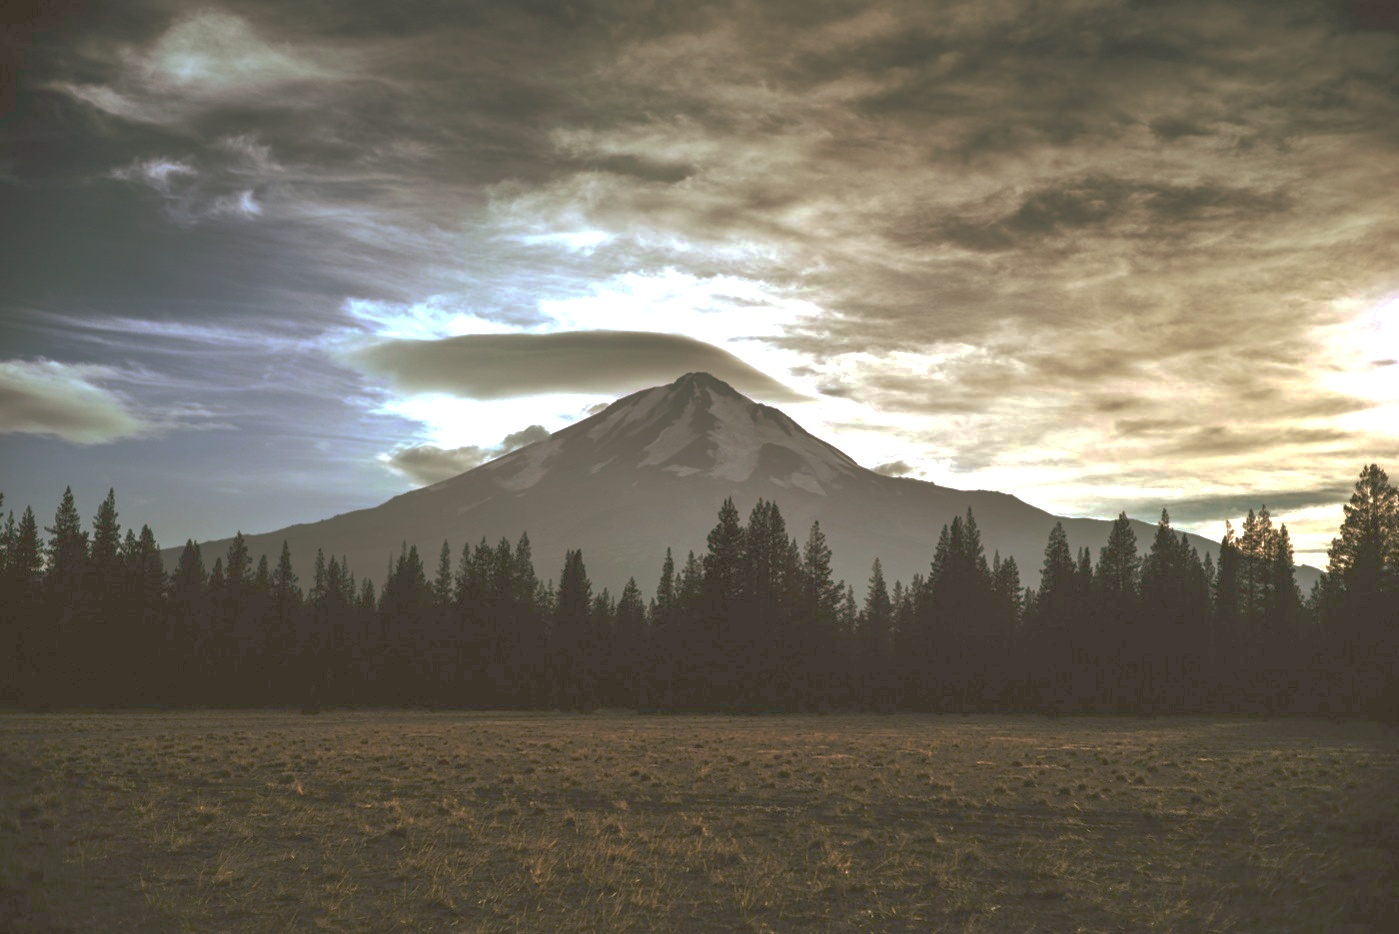
\includegraphics[width=0.56\textwidth]{images/5exponential/photo.jpg}
    \begin{minipage}{0.5\textwidth}
        \centering 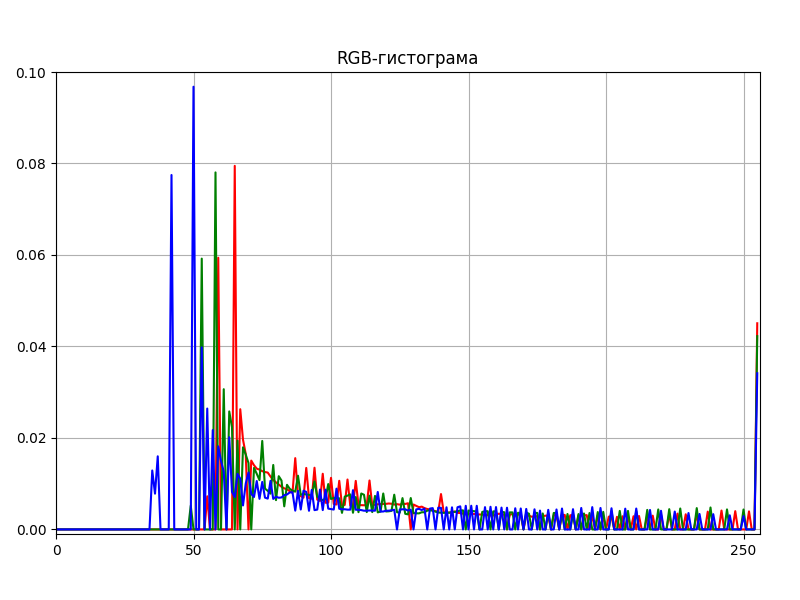
\includegraphics[width=\textwidth]{images/5exponential/hist.png}
    \end{minipage}\hfill
    \begin{minipage}{0.5\textwidth}
        \centering 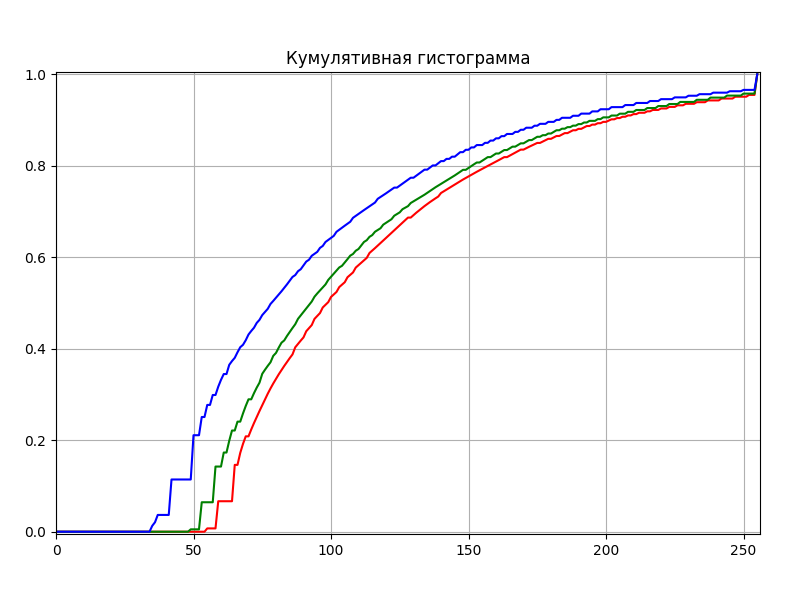
\includegraphics[width=\textwidth]{images/5exponential/cumhist.png}
    \end{minipage}
\end{figure}\noindent
Изображение стало гораздо темнее, но при этом детали елей ещё различимы, а небо выглядит более детализированным, как и трава на поле. При этом виньетка вокруг изображения стала меньше, а на небе видны яркие пятна. Преобразование хорошо подойдёт для тёмных изображений с широким диапазоном.


\newpage\addsubsection{Преобразование по закону Рэлея}
\textbf{Преобразование по закону Рэлея} --- это преобразование, которое подгоняет RGB-гистограмму так, что кумулятивная гистограмма становится функцией Рэлея, причём угол наклона функции можно регулировать с помощью коэффициента $\alpha = 0.4$. А теперь посмотрим на код этого преобразования:
\begin{lstlisting}[language=Python, caption={Код, реализующий преобразование по закону Рэлея}]
def rayleigh_conversion(image: MatLike, alpha: float) -> NDArray[np.uint8]:
    """Преобразование гистограммы по закону Рэлея"""
    channels = cv2.split(image)
    cumhists = calc_cumulative_hist(channels)
    new_channels = []
    for channel, cumhist in zip(channels, cumhists):
        cmin = channel.min()
        new_channels.append(cmin + np.sqrt(2 * alpha**2 * np.log(1 / (1 - cumhist[channel]))) * 255)
    return cv2.merge(new_channels)


apply_method(rayleigh_conversion, image, '6rayleigh', alpha=0.4)
\end{lstlisting}
\begin{figure}[H]
    \centering
    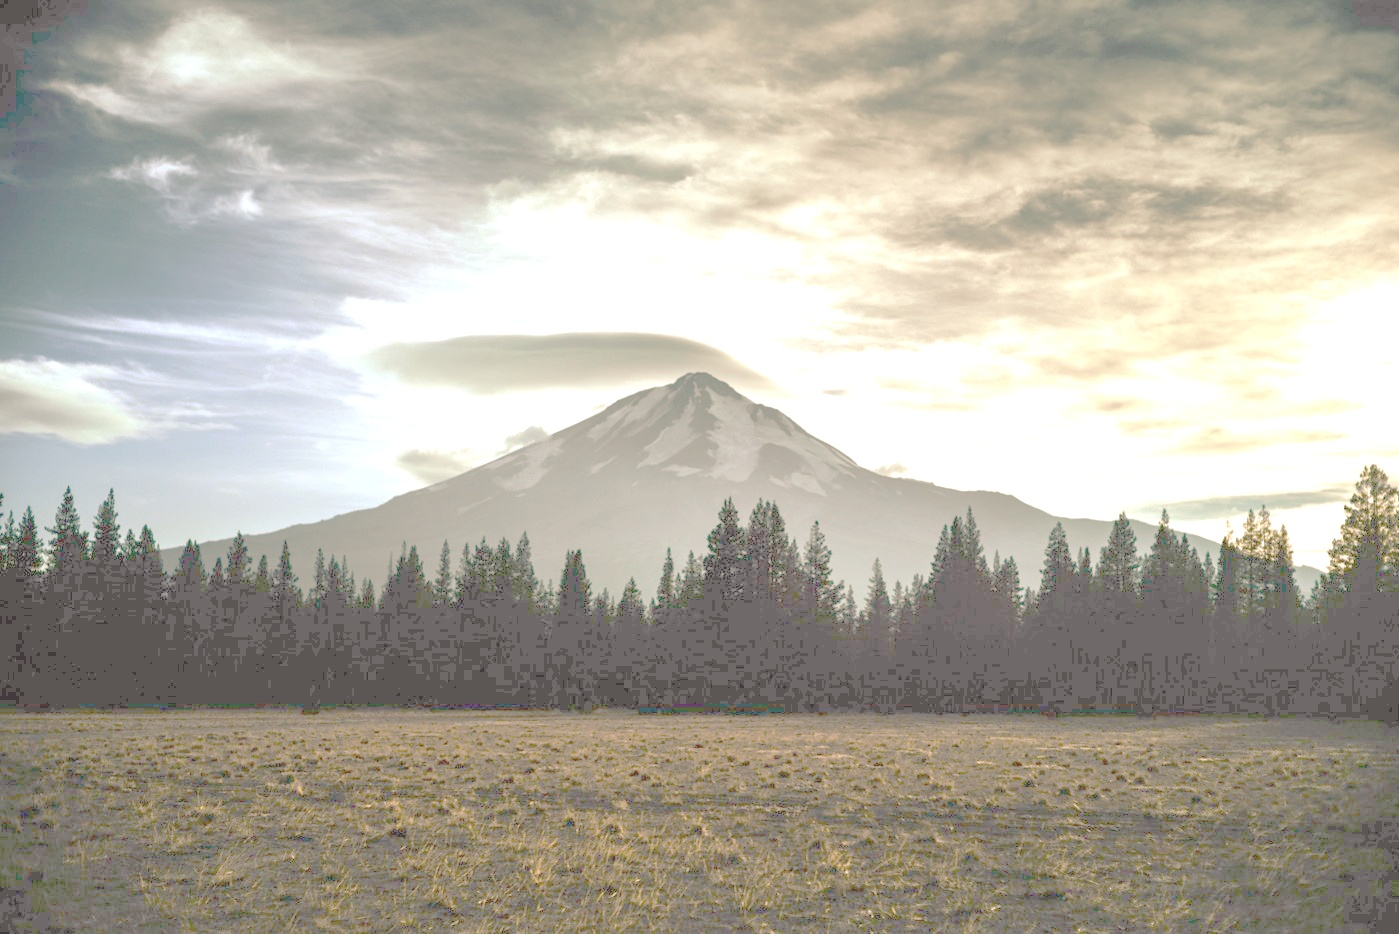
\includegraphics[width=0.56\textwidth]{images/6rayleigh/photo.jpg}
    \begin{minipage}{0.5\textwidth}
        \centering 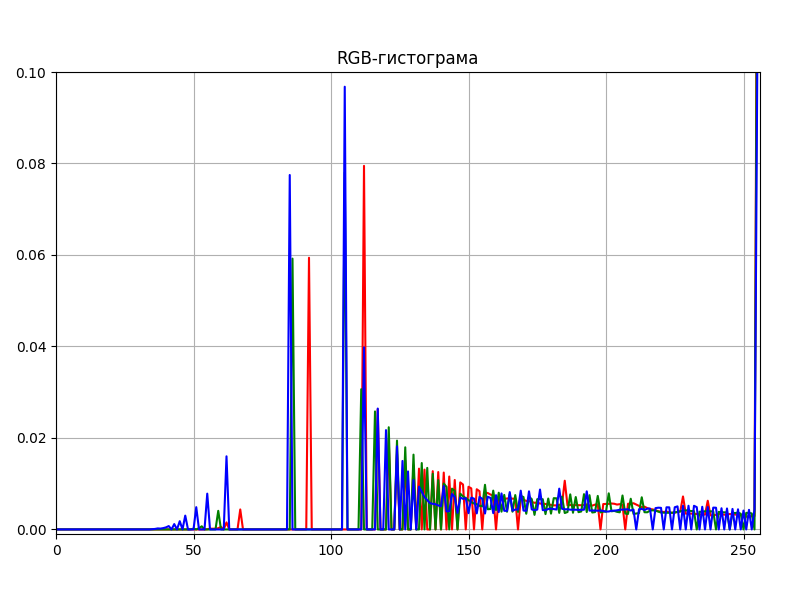
\includegraphics[width=\textwidth]{images/6rayleigh/hist.png}
    \end{minipage}\hfill
    \begin{minipage}{0.5\textwidth}
        \centering 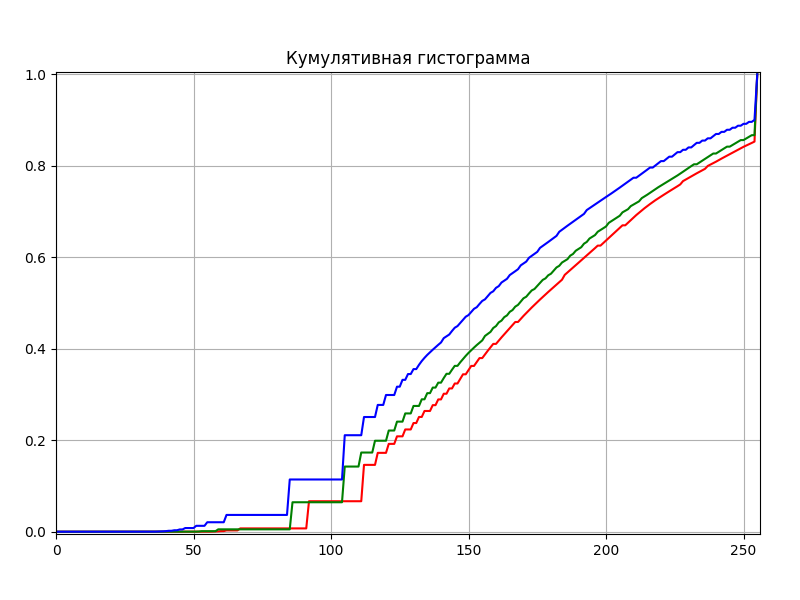
\includegraphics[width=\textwidth]{images/6rayleigh/cumhist.png}
    \end{minipage}
\end{figure}\noindent
Сразу видно, что изображение стало сильно ярче, при этом много деталей на светлых участках неба упущено. Но тёмные участки изображения стали более контрастными, что отличает преобразование по закону Рэлея от обычных арифметических операций, лишь изменяющих яркость изображение. Преобразование подойдёт для тёмных изображений с узким диапазоном, но не для ярких изображений и не для широкого диапазона.


\newpage\addsubsection{Преобразование по законку степени $\nicefrac{2}{3}$}
\textbf{Преобразование по закону степени} $\nicefrac{\mathbf{2}}{\mathbf{3}}$ --- это преобразование, которое подгоняет RGB-гистограмму так, что кумулятивная гистограмма становится показательной функцией степени $\nicefrac{2}{3}$. Рассмотрим код этого преобразования:
\begin{lstlisting}[language=Python, caption={Код, реализующий преобразование по законку степени $\nicefrac{2}{3}$}]
def rule23_conversion(image: MatLike) -> NDArray[np.uint8]:
    """Преобразование гистограммы по закону степени 2/3"""
    channels = cv2.split(image)
    cumhists = calc_cumulative_hist(channels)
    new_channels = []
    for channel, cumhist in zip(channels, cumhists):
        new_channels.append(cumhist[channel] ** (2 / 3) * 255)
    return cv2.merge(new_channels)


apply_method(rule23_conversion, image, '7rule23')
\end{lstlisting}
\begin{figure}[H]
    \centering
    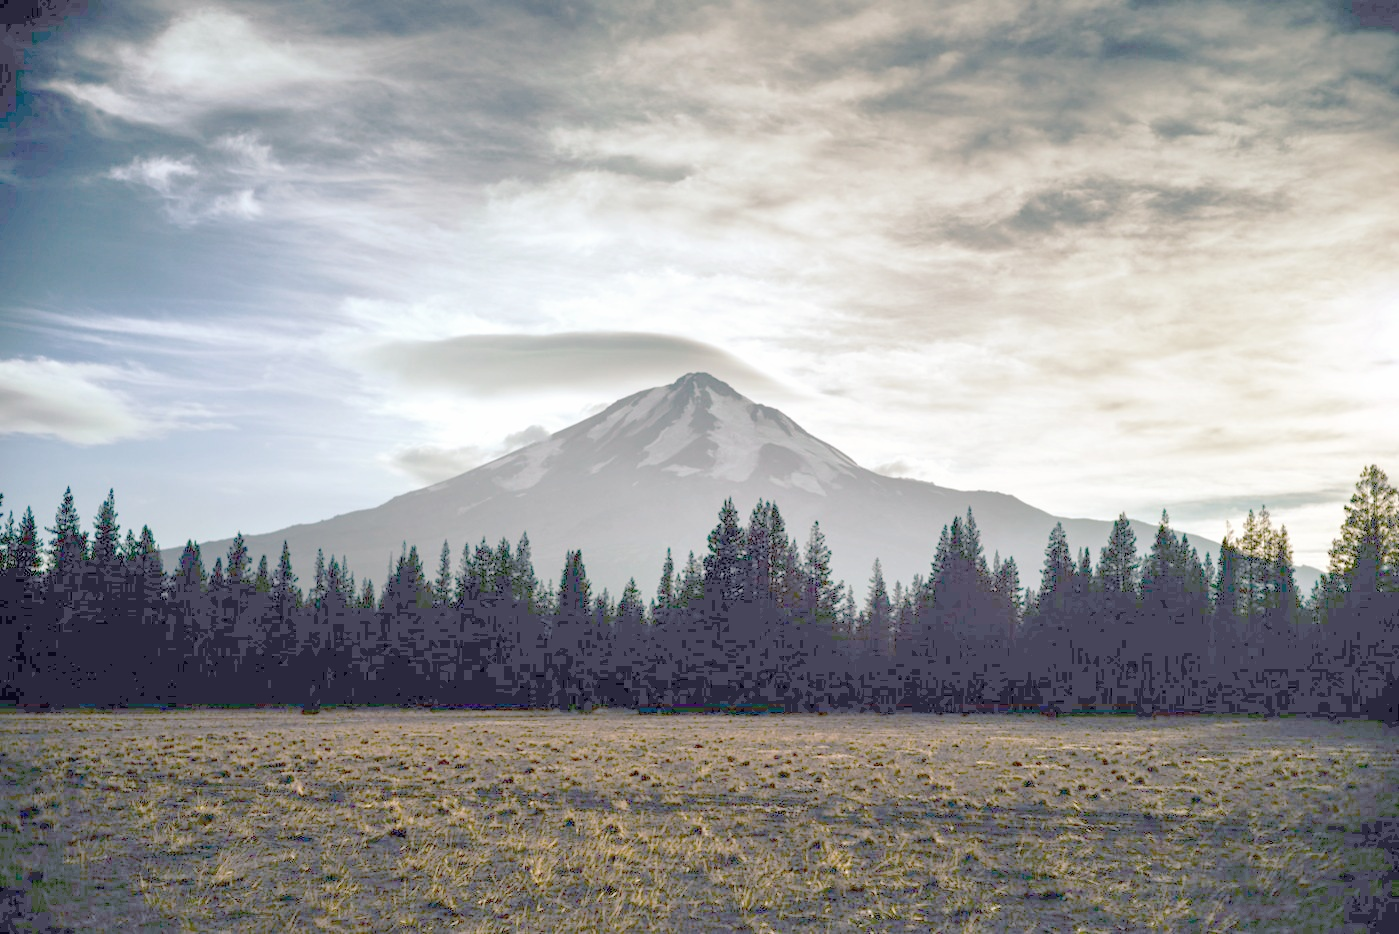
\includegraphics[width=0.56\textwidth]{images/7rule23/photo.jpg}
    \begin{minipage}{0.5\textwidth}
        \centering 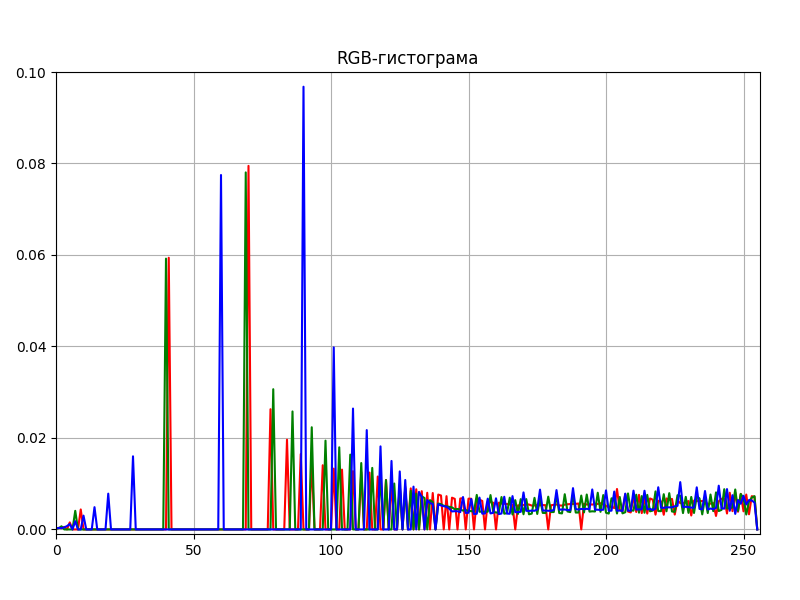
\includegraphics[width=\textwidth]{images/7rule23/hist.png}
    \end{minipage}\hfill
    \begin{minipage}{0.5\textwidth}
        \centering 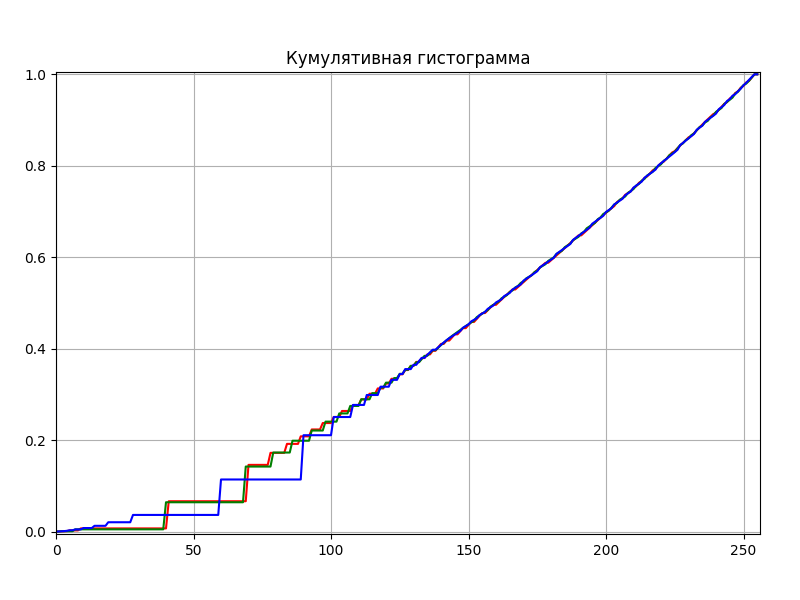
\includegraphics[width=\textwidth]{images/7rule23/cumhist.png}
    \end{minipage}
\end{figure}\noindent
Преобразование очень похоже на линейное выравнивание, но при этом оно более нелинейное, что добавляет в яркости и в контрастности, но вносит небольшие искажения в тёмные участки. Это преобразование подойдёт к более тёмным и детализированным изображениям, но не к ярким и с высокой контрастностью. 


\newpage\addsubsection{Гиперболическое преобразование}
\textbf{Гиперболическое преобразование} --- это преобразование, которое подгоняет RGB-гистограмму так, что кумулятивная гистограмма становится похожа на гиперболу в четвёртой четверти декартовой системы координат. Ввиду того, что в формуле показательная функция, в отличие от, например, предыдущего преобразования, мы получим довольно неожиданный результат. И вот как выглядит код этого преобразования:
\begin{lstlisting}[language=Python, caption={Код, реализующий гиперболическое преобразование}]
def hyperbolic_conversion(image: MatLike, alpha: float) -> NDArray[np.uint8]:
    """Преобразование гистограммы по закону степени 2/3"""
    channels = cv2.split(image)
    cumhists = calc_cumulative_hist(channels)
    new_channels = []
    for channel, cumhist in zip(channels, cumhists):
        new_channels.append(alpha ** cumhist[channel] * 255)
    return cv2.merge(new_channels)


apply_method(hyperbolic_conversion, image, '8hyperbolic', alpha=0.04)
\end{lstlisting}
\begin{figure}[H]
    \centering
    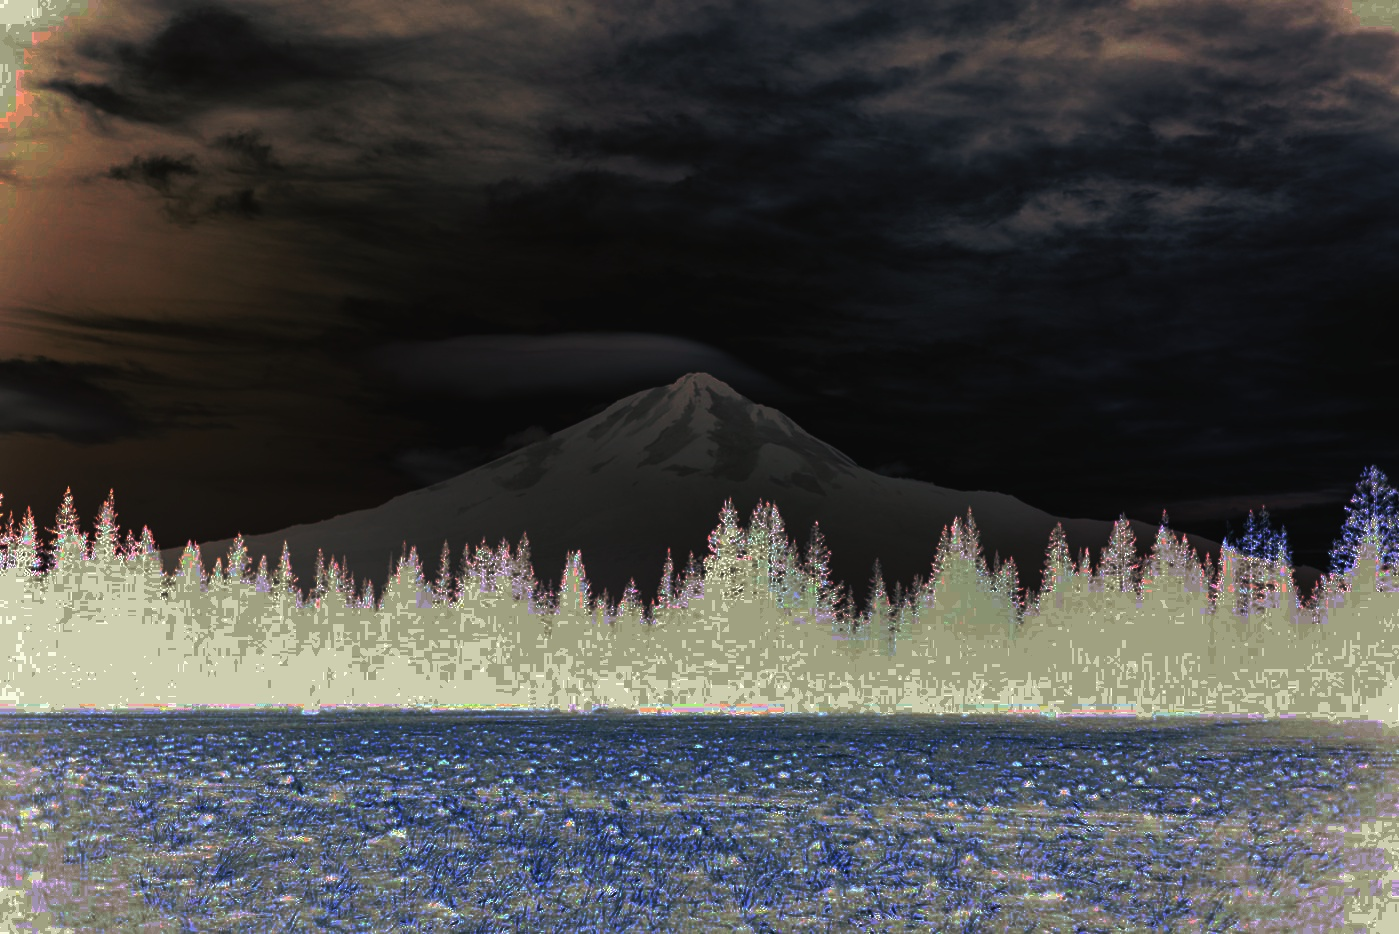
\includegraphics[width=0.56\textwidth]{images/8hyperbolic/photo.jpg}
    \begin{minipage}{0.5\textwidth}
        \centering 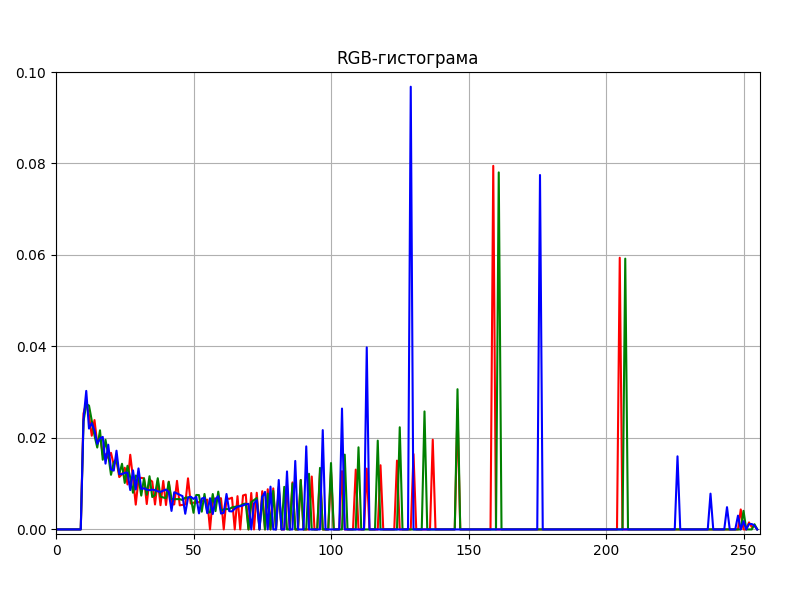
\includegraphics[width=\textwidth]{images/8hyperbolic/hist.png}
    \end{minipage}\hfill
    \begin{minipage}{0.5\textwidth}
        \centering 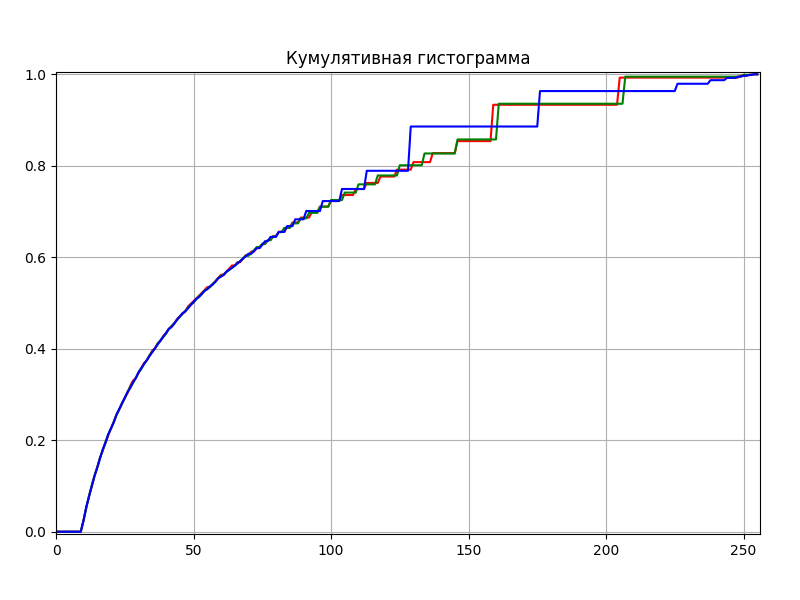
\includegraphics[width=\textwidth]{images/8hyperbolic/cumhist.png}
    \end{minipage}
\end{figure}\noindent
Глубину получившегося негатива можно регулировать, изменяя $\alpha = 0.04$ --- этот коэффициент влияет на крутизну гиперболы и на яркость и контраст изображения. Такой негатив подойдёт для отделения фона от объекта на изображении и для его анализа, но, конечно, здесь не идёт речи об улучшении визуального качества изображения.


\newpage\addsubsection{Таблица поиска}
\textbf{Таблица поиска} --- это метод для преобразования интенсивности пикселей изображения с помощью таблицы преобразования. В данном случае мы применим таблицу преобразования, которая будет преобразовывать интенсивность пикселей изображения по степенному закону с коэффициентом $\alpha = 0.5$. Рассмотрим код этого преобразования:
\begin{lstlisting}[language=Python, caption={Код, применяющий таблицу поиска к изображению}]
def LUT_conversion(image: MatLike, alpha: float) -> NDArray[np.uint8]:
    """Преобразование изображения с помощью таблицы преобразования"""
    lut = np.arange(256, dtype=np.uint8)
    lut = (lut - image.min()) / (image.max() - image.min())
    lut = np.where(lut > 0, lut, 0)
    lut = np.clip(255 * np.power(lut, alpha), 0, 255)
    return cv2.LUT(image, lut)


apply_method(LUT_conversion, image, '9LUT', alpha=0.5)
\end{lstlisting}
\begin{figure}[H]
    \centering
    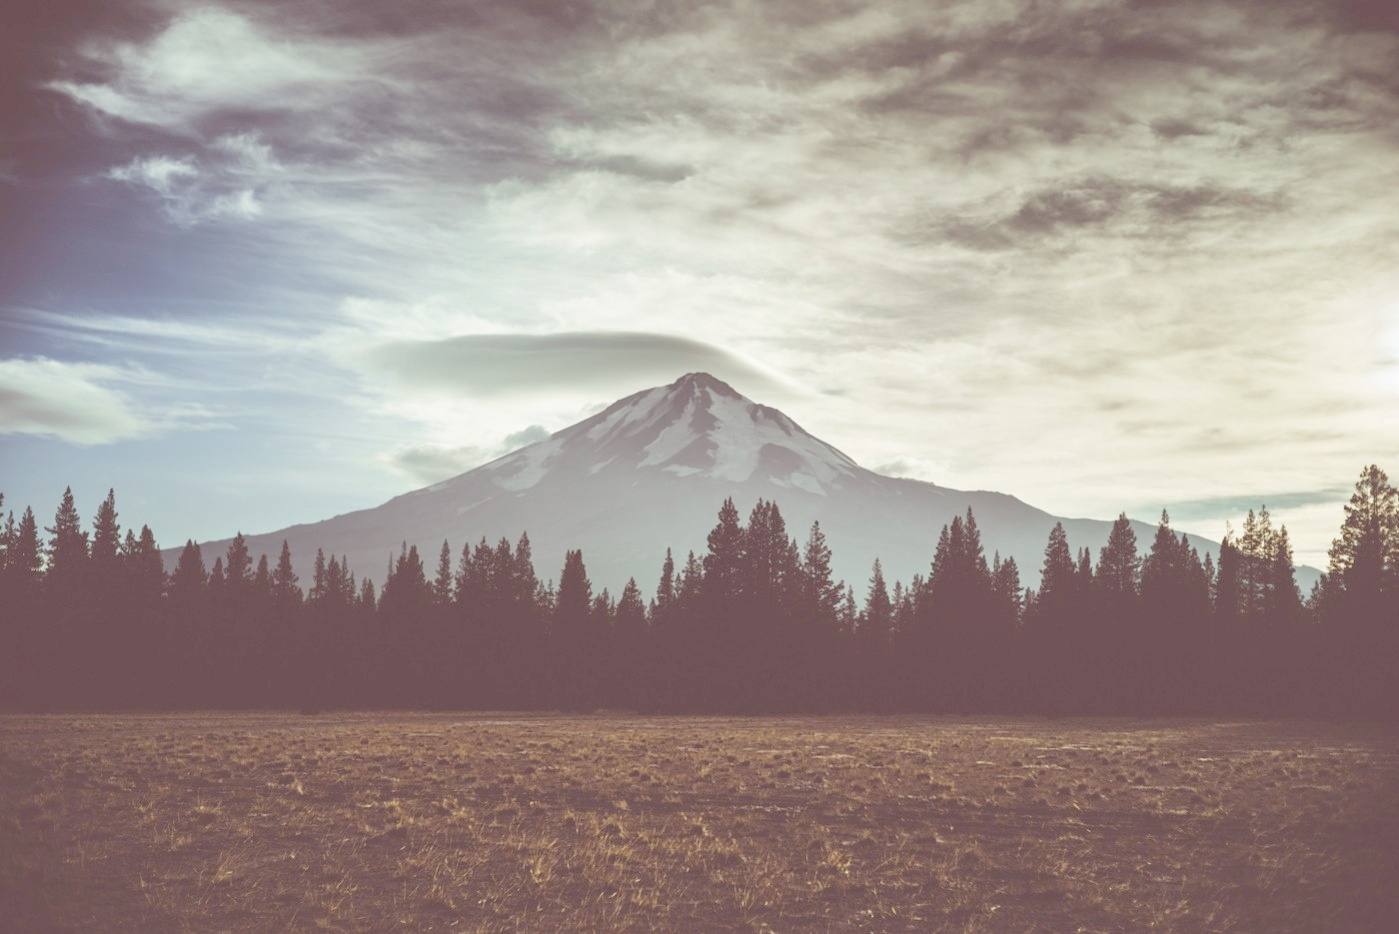
\includegraphics[width=0.56\textwidth]{images/9LUT/photo.jpg}
    \begin{minipage}{0.5\textwidth}
        \centering 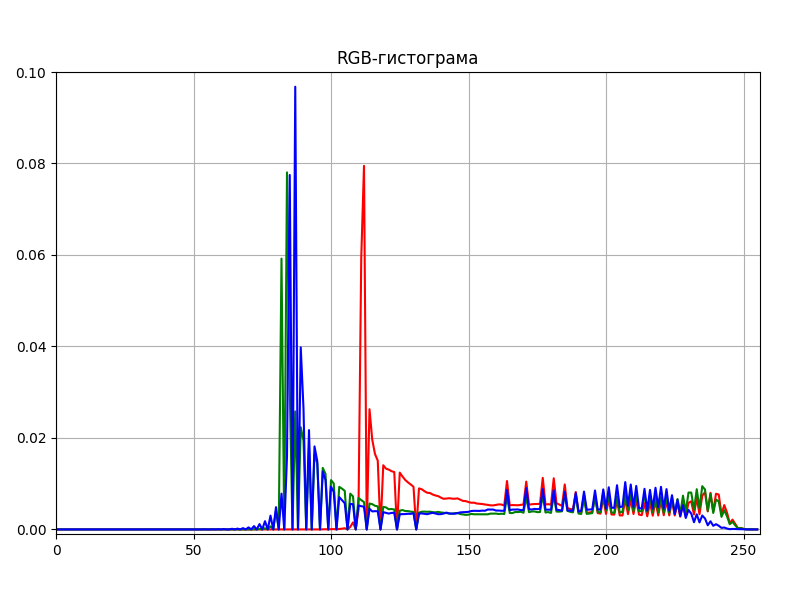
\includegraphics[width=\textwidth]{images/9LUT/hist.png}
    \end{minipage}\hfill
    \begin{minipage}{0.5\textwidth}
        \centering 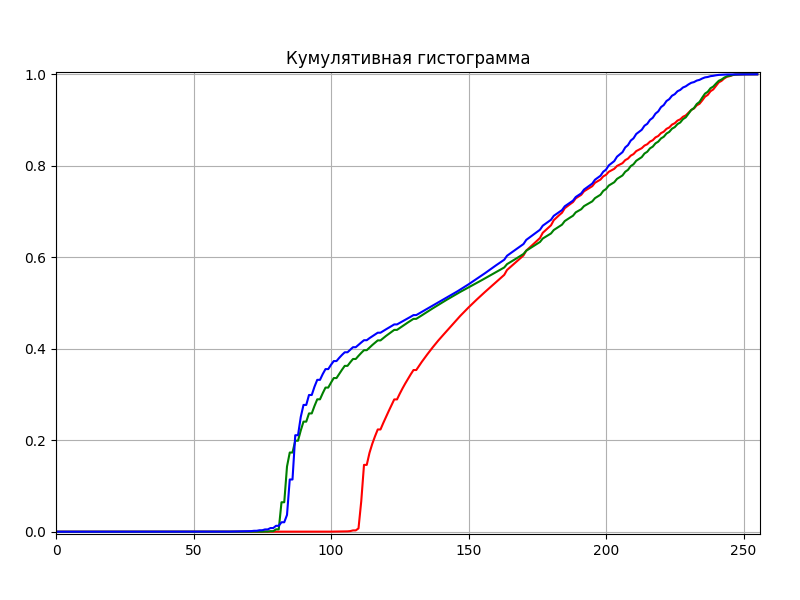
\includegraphics[width=\textwidth]{images/9LUT/cumhist.png}
    \end{minipage}
\end{figure}\noindent
По RGB-гистограмме видно, что на тёмных градациях произошло разрежение гистограммы, а на светлых --- наоборот, интенсивность приподнялась, при этом вся гистограмма сдвинулась вправо, что сделало изображение в целом ярче. Изображение воспринимается легче и на нём видно больше деталей благодаря поднятию интенсивности светлых пикселей. Преобразование подойдёт для любых изображений, т.к. таблица поиска строится индвидуально для каждого изображения, но там, где плюсы, там и минусы --- не стоит ожидать сверхъестественного улучшения визуального качества. 

\newpage\addsection{Профили и проекции}
\addsubsection{Профиль изображения вдоль горизонтальной линии по середине}
\textbf{Профилем изображения} называют функцию интенсивности изображения, распределённой вдоль некоторой линии (представьте себе сканер, который сканирует полоску шириной в 1 пиксель). В данном случае мы рассмотрим профиль изображения вдоль горизонтальной линии по середине изображения. Вот код для отображения профиля изображения: 
\begin{lstlisting}[language=Python, caption={Код, отображающий профиль изображения}]
def render_image_profile(img: MatLike, name: str):
    """Рендерит профиль яркости изображения"""
    clear()
    profile = img[img.shape[0] // 2, :]

    fig = plt.figure()
    fig.set_size_inches(654 / fig.dpi, 744 / fig.dpi)

    ax1 = plt.subplot2grid((2, 1), (0, 0))
    ax1.set_title('Исходное изображение')
    ax1.imshow(cv2.cvtColor(img, cv2.COLOR_BGR2RGB), aspect='auto')

    ax2 = plt.subplot2grid((2, 1), (1, 0), sharex=ax1)
    ax2.set_xlabel('Профиль яркости', fontsize='large')
    ax2.plot(profile)
    plt.setp(ax2.get_xticklabels(), visible=False)

    plt.savefig(f'{name}_profile.png')


barcode_image = cv2.imread('barcode.png')
render_image_profile(barcode_image, 'barcode')
\end{lstlisting}
\begin{figure}[H]
    \centering
    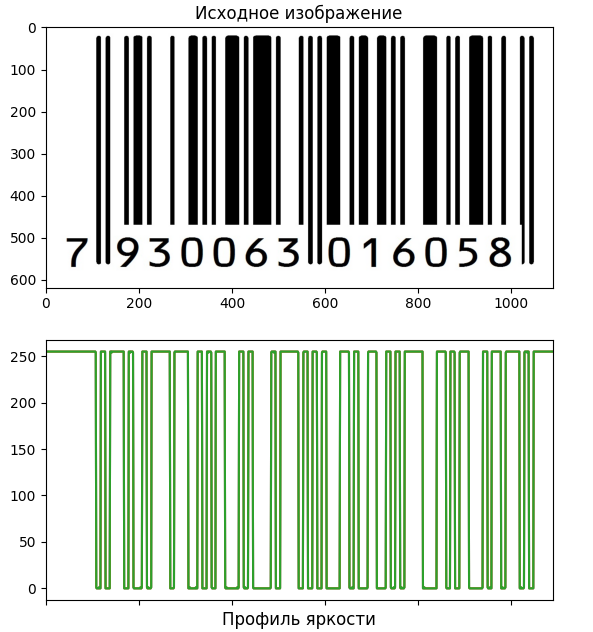
\includegraphics[width=0.5\textwidth]{images/barcode_profile.png}
\end{figure}\noindent
Результат на лицо, профиль изображения помогает в распознавании штрихкодов и QR-кодов, анализе медицинских изображений и текстур или в измерении контраста. И мы отчётливо видим, как профиль резкими перепадами показывает тёмные участки изображения --- по сути полосы штрихкода.


\newpage\addsubsection{Проекция изображения на оси}
\textbf{Проекция изображения} на ось --- сумма интенсивности пикселей изображения в направлении, перпендикулярном этой оси (представьте, как прозрачный шарик катится по прямой линии и чем сильнее он будет окрашен в цвета изображения в конце пути, тем выше значение на графике). Рассмотрим проекции изображения на горизонтальную и вертикальную оси. Перед вами код для отображения этих проекций:
\begin{lstlisting}[language=Python, caption={Код, отображающий проекции изображения на обе оси}]
def render_projection(img: MatLike, name: str):
    """Рендерит проекцию изображения"""
    clear()
    channels = cv2.split(img)
    projection_x = sum(np.sum(channel, axis=0) for channel in channels) / img.shape[0] / 3
    projection_y = sum(np.sum(channel, axis=1) for channel in channels) / img.shape[1] / 3

    fig = plt.figure()
    fig.set_size_inches(600 / fig.dpi, 840 / fig.dpi)

    ax1 = plt.subplot2grid((3, 3), (0, 0), rowspan=2, colspan=2)
    ax1.set_title('Исходное изображение')
    ax1.imshow(cv2.cvtColor(img, cv2.COLOR_BGR2RGB), aspect='auto')

    ax2 = plt.subplot2grid((3, 3), (2, 0), colspan=2, sharex=ax1)
    ax2.set_xlabel('Проекция на X', fontsize='large')
    ax2.plot(range(img.shape[1]), projection_x)
    plt.setp(ax2.get_xticklabels(), visible=False)

    ax3 = plt.subplot2grid((3, 3), (0, 2), rowspan=2, sharey=ax1)
    ax3.set_title('Проекция на Y')
    ax3.plot(projection_y, range(img.shape[0]))
    plt.setp(ax3.get_yticklabels(), visible=False)

    plt.savefig(f'{name}_projection.png')


passport_image = cv2.imread('passport.jpg')
render_projection(passport_image, 'passport')
\end{lstlisting}
\begin{figure}[H]
    \centering
    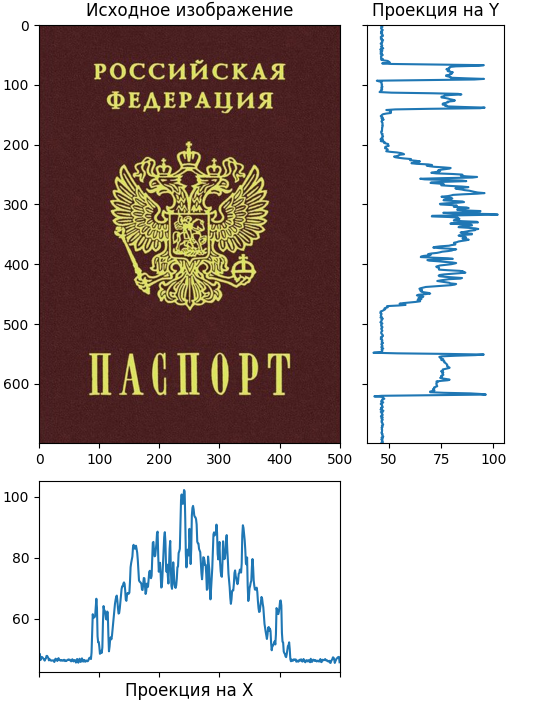
\includegraphics[width=0.4\textwidth]{images/passport_projection.png}
\end{figure}\noindent
Делаем вывод, что проекции полезны для анализа шаблонов и выделения отдельных объектов на монотонном изображении с получением их размеров и с последующим их обрезанием.


\newpage\addsection{Вывод}
В этой лабораторной работе мы освоили методы преобразования изображения для изменения его характеристик и улучшения визуального качества, чтобы в последующем упростить анализ изображения. Кроме того, мы изучили профили и проекции изображения, которые также помогают в анализе изображения и благодаря которым мы сможем выделять границы и объекты на изображении. К тому же мы познакомились с библиотекой \verb|OpenCV| и библиотекой \verb|Matplotlib|, которые упрощают работу с изображениями и визуализацией результаты --- всё это помогло нам лучше понять, как работают представленные преобразования. В целом, лабораторная работа прошла успешно, и мы готовы двигаться дальше.\\[0.5em]
Напомним, что весь код из этой лабораторной работы и в том числе для генерации гистограмм и результатов можно найти в \href{https://gist.github.com/PaveTranquil/64ed1c48f4faa3a25f826c5f00c7ab5f}{приватном гисте в GitHub}.

\addsection{Вопросы к защите}
\begin{enumerate}
    \item Что такое контрастность изображения и как её можно изменить?
    \begin{quotebox}
        Контрастность изображения --- это интервал между самым тёмным и самым ярким пикселем изображения. Её можно изменить с помощью различных преобразований, выбрав наиболее подходящие для конкретного изображения.
    \end{quotebox}
    \item Чем эффективно использование профилей и проекций изображения?
    \begin{quotebox}
        Профили и проекции изображения помогают в определении границ и размеров объектов на монотонном изображении, а также в анализе шаблонов и обрезании изображений.
    \end{quotebox}
    \item Каким образом можно найти объект на равномерном фоне?
    \begin{quotebox}
        Можно использовать проекции изображения на одну из осей, чтобы найти расположение объектов, а затем с помощью профилей определить форму и границы объекта на двумерной плоскости, чтобы выделить его.
    \end{quotebox}
\end{enumerate}
\end{document}